\documentclass[a4paper]{article}
\usepackage{graphicx}
\usepackage{natbib}
\usepackage{vmargin}
\usepackage{amsmath}
\usepackage{amsfonts}
\usepackage{lmodern}
\usepackage{fix-cm}
\usepackage{bbm}
\usepackage{hyperref}

\title{\texttt{bdsm}: Bayesian dynamic systems modelling. \\ Bayesian model averaging for dynamic panels \\ with weakly exogenous regressors}
\author{Krzysztof Beck \\ Lazarski University
\and Marcin Dubel \\ Lazarski University
\and Mateusz Wyszyński \\ Lazarski University \\ University of Warsaw}

\usepackage{Sweave}
\begin{document}
\Sconcordance{concordance:bdsm_vignette.tex:bdsm_vignette.Rnw:1 16 1 1 0 364 1 1 2 4 %
0 1 2 3 1 1 2 4 0 1 2 5 1 1 2 21 0 1 2 2 1 1 2 21 0 1 2 3 1 1 5 7 0 1 2 %
11 1 1 5 7 0 1 2 5 1 1 8 10 0 1 2 103 1 1 2 1 0 2 1 3 0 1 2 15 1 1 2 4 %
0 1 2 9 1 1 2 4 0 1 2 5 1 1 2 17 0 1 2 18 1 1 2 17 0 1 2 11 1 1 2 9 0 1 %
2 16 1 1 2 5 0 1 2 3 1 1 2 5 0 1 2 16 1 1 2 5 0 1 2 25 1 1 2 1 0 1 1 17 %
0 1 2 3 1 1 2 1 0 1 1 18 0 1 2 6 1 1 2 1 0 1 1 7 0 1 2 10 1 1 2 16 0 1 %
2 7 1 1 2 16 0 1 2 5 1 1 2 16 0 1 2 15 1 1 2 1 0 1 1 4 0 1 2 1 1 1 2 1 %
0 1 1 4 0 1 2 1 1 1 2 1 0 1 2 5 0 1 2 15 1 1 3 5 0 1 2 2 1 1 2 9 0 1 2 %
3 1 1 2 5 0 1 2 4 1 1 2 5 0 1 2 4 1 1 2 17 0 1 2 5 1 1 2 17 0 1 2 5 1 1 %
2 16 0 1 2 4 1 1 3 2 0 1 1 8 0 1 2 2 1 1 2 5 0 1 2 3 1 1 2 5 0 1 2 3 1 %
1 2 17 0 1 2 4 1 1 2 17 0 1 2 5 1 1 2 16 0 1 2 13 1 1 3 5 0 1 2 2 1 1 2 %
5 0 1 2 5 1 1 3 2 0 1 1 4 0 1 2 2 1 1 3 2 0 1 1 4 0 1 2 4 1 1 2 17 0 1 %
2 26 1}

%\setpapersize{A4}
% \VignetteIndexEntry{bdsm: Bayesian dynamic systems modelling}
\maketitle
\abstract{This manuscript introduces the \verb+bdsm+ package, which enables Bayesian model averaging for dynamic panels with weakly exogenous regressors—a methodology developed by \citet{Moral+2016}.
The package allows researchers to simultaneously address model uncertainty and reverse causality.
The manuscript includes a hands-on tutorial accessible to users unfamiliar with this approach.
In addition to calculating the model space (using parallel computing) and providing key BMA statistics, the package offers flexible options for specifying model priors, including a dilution prior that accounts for multicollinearity.
It also provides graphical tools for visualizing prior and posterior model probabilities, as well as functions for plotting histograms and kernel densities of the estimated coefficients.
Furthermore, the package enables researchers to compute jointness measures and perform Bayesian model selection to examine the most probable models based on posterior model probabilities.}


\tableofcontents

\clearpage
\section{Introduction}

Since the seminal works of \citet{Leamer+1978,Leamer+1981,Leamer+1983,Leamer+1985}, there has been an increased focus on reporting the fragility of regression estimates.
\citet{Leamer+1983} proposed Extreme Bounds Analysis (EBA) as a remedy for addressing the sensitivity of empirical research findings\footnote{\citet{Hlavac+2016} developed an R package for EBA.}.
In economics, growth regressions \citep{Barro+1991} became a central focus of research on economic growth during the 1990s.
However, the credibility of these results was challenged when \citet{Levine+1992} applied EBA to cross-country economic growth data.
The authors found that investment as a share of GDP was the only variable robust to changes in model specification.
In response, EBA was criticized for being too stringent\footnote{\citet{Granger+1990} proposed a less restrictive variant of EBA.}, leading to the proposal of alternative approaches \citep{Sala+1997}.

Bayesian model averaging (BMA) emerged as a preferred method during a period when studies of economic growth advanced alongside methodological innovations \citep{Fernandez+2001,Fernandez+2001b,Sala+2004,Eicher+2007,Ley+2012,Moser+2014,Fernandez+2001,Fernandez+2001b,Arin+2019}.
As a result, BMA became a widely used technique for assessing the robustness of regressors in economics\footnote{For a detailed review of BMA applications in economics, see \citet{Moral+2015,Steel+2020}.} (e.g., \citet{Liu+2009,Ductor+2016,Figini+2017,Beck+2022,DAndrea+2022,Horvath+2024}), as well as in other fields (e.g., \citet{Sloughter+2013,Baran+2015,Aller+2021,Guliyev+2024,Payne+2024}).
Moreover, the growing interest in BMA was fueled by the availability of R packages such as \verb+BMA+ \citep{Raftery+2005}, \verb+BAS+ \citep{clyde2011bayesian}, and \verb+BMS+ \citep{Feldkircher+2015}, along with the \verb+gretl+ BMA package developed by \citet{Blazejowski+2015}.

The primary issue with the Bayesian model averaging in the aforementioned studies was its reliance on the assumption of exogenous regressors.
In many contexts, particularly in economics, this premise is unsuitable.
Instead, the assumption of endogenous variables within a simultaneous equations framework is more fitting.
Consequently, a new line of research relaxed the assumption of exogenous regressors \citet{Lenkoski+2014,Leon+2015,Mirestean+2016,Moral+2016,Chen+2018}.
However, these methods have not found their way into mainstream research.
The code to implement them is only available upon request from the authors and is provided exclusively for \verb+MATLAB+ and \verb+GAUSS+.

The \verb+bdsm+ package was developed to address this gap.
It offers tools for performing Bayesian model averaging on dynamic panels with weakly exogenous regressors.
As a result, it enables researchers to address both model uncertainty and reverse causality.
The core of the code is based on the methodological approach developed by \citet{Moral+2012,Moral+2013,Moral+2016}.
While the main aspects of the method are described in the manuscript, interested readers should refer to the original articles for further details.
In addition to the key features developed by \citet{Moral+2016}, the \verb+bdsm+ package offers a wide range of additional functionalities.
The package enables users to employ flexible model prior options, along with a dilution prior, which helps account for multicollinearity.
The \verb+bdsm+ package provides users with graphical options for plotting prior and posterior model probabilities across model sizes and the model space.
Additionally, users can utilize Bayesian model selection to thoroughly examine the best models based on posterior model probability.
The package calculates jointness measures developed by \citet{Doppelhofer+2009,Ley+2007,Hofmarcher+2018}.
Finally, it offers users the option to plot histograms or kernel densities of the estimated coefficients for the examined regressors.

The remainder of the manuscript is structured as follows.
Section \ref{ms_bma} describes the dynamic panel setup considered by \citet{Moral+2013} and outlines the Bayesian model averaging approach used in the package.
Data preparation is detailed in Section \ref{data}, while Section \ref{model_space} addresses the estimation of the model space.
Section \ref{using_bma} provides an overview of the \verb+bdsm+ functions related to performing Bayesian model averaging, calculating jointness measures, and presenting the estimation results.
The details of the model prior choices are described in Section \ref{priors}.
Finally, Section \ref{sum} offers some concluding remarks.



\section{Model setup and Bayesian model averaging}\label{ms_bma}
This section outlines the model setup, describes the approach to Bayesian model averaging implemented in the package, summarizes the main BMA statistics, and discusses model priors and jointness measures.

\subsection{Model setup}
\noindent \citet{Moral+2016} considers the following model specification:
\begin{equation}\label{eq1}
    y_{it}=\alpha y_{it-1}+\beta x_{it}+\eta_{i}+\zeta_{t}+v_{it}
\end{equation}
\noindent where $y_{it}$ is the dependent variable, $i$ $(=1,...,N)$ indexes entity (ex. country), $t$ $(=1,...,T)$ indexes time, $x_{it}$ is a matrix of growth determinants, $\beta$ is a parameter vector, $\eta_{i}$ is an entity specific fixed effect, $\zeta_{t}$ is a period-specific shock and $v_{it}$ is a shock to the dependent variable.
To address the issue of reverse causality the model is build on the assumption of weak exogeneity, that can be formalized as
\begin{equation}\label{eq2}
    \mathbb{E}(v_{i,t}|y^{t-1}_{t},x^{t}_{i},\eta_{i})=0
\end{equation}
\noindent where $y^{t-1}_{t}=(y_{i,0},...,y_{i,t-1})'$ and $x^t_{i}=(x_{i,0},...,x_{i,t})'$.
Accordingly, weak exogeneity implies that the current values of the regressors, lagged dependent variable, and fixed effects are uncorrelated with the current shocks, while they are all allowed to be correlated with each other at the same time.
On the assumption of weakly exogenous regressors, \citet{Moral+2013} augmented equation (\ref{eq1}) with additional reduced-form equations capturing the unrestricted feedback process:
\begin{equation}\label{eq3}
x_{it}=\gamma_{t0}y_{i0}+...+\gamma_{tt-1}y_{it-1}+\Lambda_{t1}x_{i1}+...+\Lambda_{tt-1}x_{it-1}+c_{t}\eta_{i}+\vartheta_{it}
\end{equation}
\noindent where $t=2,\dots ,T;$ $c_{t}$ is the $k\times 1$ vector of parameters.
For $h<t$, $\gamma_{th}$ is a $k\times 1$ vector $(y_{th}^{1},\dots,y_{th}^{k})'$  $h=0,\dots,T-1$; $\Lambda_{th}$ is a $k\times k$ matrix of parameters, and $\vartheta_{it}$ is a $k\times 1$ of prediction errors. The initial observations are defined with
\begin{equation}\label{eq4}
    y_{i0}=c_{0}\eta_{i}+\upsilon_{it}
\end{equation}
\begin{equation}\label{eq5}
    x_{i1}=\gamma_{10}y_{i0}+c_{1}\eta_{i}+\vartheta_{it}
\end{equation}
\noindent where $c_{0}$ is a scalar, $c_{1}$ and $\gamma_{10}$ are $k\times 1$ vectors and $\eta_{i}$ are the individual effects. The mean vector and the covariance matrix of the joint distribution of the initial observations and the individual effects are unrestricted.\footnote{The method outperforms the Arellano--Bond estimator \citep{Moral+2019}.}
\indent For the model setup given in equations (\ref{eq1}) and (\ref{eq3}-\ref{eq5}), \citet{Moral+2013} derived the log-likelihood function:
\begin{equation}\label{eq6}
    \log f(data|\theta) \propto \frac{N}{2}\log\det(B^{-1}D\Sigma D'B'^{-1})-\frac{1}{2}\sum_{i=1}^{N}\{R'_{i}(B^{-1}D\Sigma D'B'^{-1})^{-1}R_{i}\}
\end{equation}
\noindent where $\theta$ denotes parameters to be estimated, $R_{i}=(y_{io},x'_{i1},y_{i1},\dots,x'_{iT},y_{iT})'$ are vectors of observed variables, and $\Sigma=diag[\sigma^{2}_{\eta},\sigma^{2}_{\upsilon_{0}},\Sigma_{\vartheta_{1}},\sigma^{2}_{\upsilon_{1}},...,\Sigma_{\vartheta_{T}},\sigma^{2}_{\upsilon_{T}}]$ is the block-diagonal variance-covariance matrix.
Matrix B is given by:
\begin{equation}\label{eq7}
B=\begin{bmatrix}
 1&0&0&0&0&\dotsc& 0&0&0\\
 -\gamma_{10}&I_{k}&0&0&0&\dotsc&0&0&0\\
 -\alpha&-\beta'&1&0&0&\dotsc&0&0&0\\
 -\gamma_{20}&-\Lambda_{21}&-\gamma_{21}&I_{k}&0&\dotsc&0&0&0\\
0&0&-\alpha&-\beta'&1&\dotsc&\vdots&\vdots&\vdots\\
\vdots&\vdots&\vdots&\vdots&\vdots&\ddots&0&0&0\\
 -\gamma_{T0}&-\Lambda_{T1}&-\gamma_{T1}&-\Lambda_{T2}&-\gamma_{T2}&\dotsc&-\gamma_{TT-1}&I_{k}&0\\
 0&0&0&0&0&\dotsc&-\alpha&-\beta'&1\\
\end{bmatrix}
\end{equation}
and matrix D is given by:
\begin{equation}\label{eq8}
D=\begin{bmatrix}
(c_{0}&c'_{1}&1&c'_{2}&1&\dotsc&c'_{T}&1)' & I_{T(k+1) + 1}
 \end{bmatrix}.
\end{equation}

\indent The model setup in equations (\ref{eq1}) and (\ref{eq3}-\ref{eq5}) requires that in addition to the parameters of interest $\alpha$ and $\beta$, the parameters $\gamma_{ij}$ and $\Lambda_{km}$ need to be estimated.
To make the optimization of likelihood computationally feasible, \citet{Moral+2013} developed Simultaneous Equations Model (SEM) setup where the parameters of non-central interest are incorporated in the variance-covariance matrix.
In the SEM setup, the model is defined by $1 + (T - 1)k + T$ equations:
\[
\begin{cases}
    \eta_i = \phi_i y_{i0} + x'_{i1} \phi_1 + \epsilon_i &  \\
    x_{it} = \pi_{t0} y_{i0} + \pi_{t1} x_{i1} + \pi^w_t x_{i1} + \xi_{it}, & t = 2, ..., T \\
    y_{it} = \alpha y_{it-1} + x'_{it} \beta + \phi_0 y_{i0} + x'_{i1} \phi_1 + w'_i \delta + \epsilon_i + v_{it}, & t = 1, ..., T
\end{cases}
\]
This setup can be rewritten in a matrix form:
\begin{equation}\label{eq9}
    B R_i = C z_i + U_i,
\end{equation}
\noindent where:
\begin{equation}\label{eq10}
    z_i = [y_{i0}, x'_{i1}, w'_i]'
\end{equation}
is the vector of strictly exogenous variables,
\begin{equation}\label{eq11}
    R_i = [y_{i1}, y_{i2}, ..., y_{iT}, x'_{i2}, x'_{i3}, ..., x'_{iT}]',
\end{equation}
\begin{equation}\label{eq12}
    U_i = [\epsilon_i + v_{i1}, \epsilon_i + v_{i2}, ..., \epsilon_i + v_{iT}, \xi'_{i2}, \xi'_{i3}, ..., \xi'_{iT}]'
\end{equation}
\noindent and matrices $B$ and $C$ contain coefficients $\alpha$, $\beta$, $\phi_0$, $\phi_1$.
Since these matrices are not connected to the error, we simply note that they are defined in such a way that the equation (\ref{eq9}) is equivalent to the SEM setup.
The main difference of the SEM setup is that equations for $x_{it}$ now depend only on $y_{i0}$ and $x_{i1}$ and not on $y_{is}$ and $x_{is}$ for other periods $s$.\\
\indent Following \citet{Moral+2013}, we can then define the likelihood function as:
\begin{equation}\label{eq13}
    L \propto - \frac{N}{2} \log \det \Omega(\theta) - \frac{1}{2} tr \{ \Omega(\theta)^{-1} (R - Z \Pi(\theta))' (R - Z \Pi(\theta)) \}
\end{equation}
where $R$ and $Z$ are matrices containing vectors $R_i$ and $z_i$ respectively and:
\begin{equation}\label{eq14}
    \Pi(\theta) = B^{-1} C
\end{equation}
\begin{equation}\label{eq15}
    U^*_i(\theta) = B^{-1} U_i
\end{equation}
\begin{equation}\label{eq16}
    \Omega(\theta) = Var(U^*_i) = B^{-1} \cdot Var(U_i) \cdot  B'^{-1} = B^{-1} \Sigma B'^{-1}
\end{equation}
It is possible to find analytical solution for MLE for some of the parameters.
Then the formula for the likelihood function can be simplified to:
\begin{equation}\label{eq17}
    L(\theta) \propto - \frac{N}{2} \log \det \Sigma_{11} - \frac{1}{2} tr \{ \Sigma_{11}^{-1} U_1' U_1 \} - \frac{N}{2} \log \det (\frac{H}{N})
\end{equation}
\normalsize
\noindent where $U_1$ is a matrix of errors connected only to dependent variables, $\Sigma_{11}$ is a part of the $\Sigma$ matrix:
\begin{equation}\label{eq18}
\Sigma=var(U_{i})=var\left(\frac{U_{i1}}{U_{i2}}\right)=\begin{bmatrix}
            \Sigma_{11}&\Sigma_{12}\\
            \Sigma_{21}&\Sigma_{22}\\
            \end{bmatrix}.
\end{equation}
\noindent and $H = (R_2 + U_1 F_{12})' Q (R_2 + U_1 F_{12})$ with $R_2$ being a matrix of regressor vectors $[x'_{i2}, x'_{i3}, ..., x'_{iT}]$ and $F_{12} = - \Sigma_{11}^{-1} \Sigma_{12}$.

\subsection{Bayesian model averaging}\label{bma}
\noindent Given the likelihood function in (\ref{eq17}), henceforth denoted as $L(\text{data}|\theta_{i}, M_{i})$ for a specific model $i$, it is possible to utilize Bayesian model averaging\footnote{For an introduction to BMA see \citet{Raftery+1995,Raftery+1997,Kass+1995b,Doppelhofer+2009,amini2011bayesian,Beck+2017,Fragoso+2018}.} (BMA).
To achieve that, we first estimate all possible variants of equation:
\begin{equation}\label{eq19}
   Y=f(X,\theta,v)
\end{equation}
\noindent where $Y$ is a vector of dependent variable, $X$ is a matrix of potential determinants, $\theta$ is a parameter vector, and $v$ is a stochastic term.
All the variants include a lagged dependent variable; therefore, with $K$ regressors, there are $2^{K}$ possible models that can be estimated.
Each of these models can be assigned a posterior model probability; however, the marginal (integrated) likelihood, $L(\text{data}|M_{i})$, must first be computed.
\citet{Moral+2012} utilizes approach of developed by \citet{Raftery+1995} and \citet{Sala+2004} based on the Bayesian information criterion (BIC) approximation.\\
\indent The Bayes factor for models $M_{i}$ and $M_{i}$, $B_{ij}=\frac{L(\text{data}|M_{i})}{L(\text{data}|M_{j})}$, can be approximated using Schwartz criterion:
\begin{equation}\label{eq20}
S=\log L(\text{data} \mid\hat{\theta_{i}},M_{i})-\log L(\text{data}|\hat{\theta_{j}},M_{j})-\frac{k_{i}-k_{j}}{2}\log (N)
\end{equation}
where $L(\text{data}|\hat{\theta}_{i}, M_{i})$ and $L(\text{data}|\hat{\theta}_{j}, M_{j})$ are the maximum likelihood values for models $i$ and $j$, respectively.
The terms $k_{i}$ and $k_{j}$ denote the number of regressors in models $i$ and $j$.
Bayesian information criterion is given by:
\begin{equation}\label{eq21}
    BIC=-2S=-2\log B_{ij}.
\end{equation}
Given null model $M_{0}$
\begin{equation}\label{eq22}
B_{ij}=\frac{L(y|M_{i})}{L(y|M_{j})}=\frac{\frac{L(y|M_{i})}{L(y|M_{0})}}{\frac{L(y|M_{j})}{L(y|M_{0})}}=\frac{B_{i0}}{B_{j0}}=\frac{B_{0j}}{B_{0i}}
\end{equation}
and
\begin{equation}\label{eq23}
2\log B_{ij}=2[\log B_{0j} - \log B_{0i}]=BIC_{j}-BIC_{i}.
\end{equation}
The posterior model probability (PMP) of model $j$ given the data is
\begin{equation}\label{eq24}
    \mathbb{P}(M_{j}|y)=\frac{L(\text{data}|M_{j})\mathbb{P}(M_{j})}{\sum_{i=1}^{2^K}L(\text{data}|M_{i})\mathbb{P}(M_{i})}
\end{equation}
where $\mathbb{P}(M_{j})$ denotes prior model probability.
In other words, the PMP represents the share of model $j$ in the total posterior probability mass.
Combining, equations (\ref{eq21}-\ref{eq24}) we get:
\begin{equation}\label{eq25}
\fontsize{9pt}{12pt} \selectfont
\begin{split}
    \mathbb{P}(M_{j}|y)=\frac{L(\text{data}|M_{j})\mathbb{P}(M_{j})}{\sum_{i=1}^{2^K}L(\text{data}|M_{i})\mathbb{P}(M_{i})}
    =\frac{\frac{L(\text{data}|M_{j})}{L(\text{data}|M_{0})}
    L(\text{data}|M_{0})\mathbb{P}(M_{j})}{\sum_{i=1}^{2^K}\frac{L(\text{data}|M_{i})}{L(\text{data}|M_{0})}
    L(\text{data}|M_{0})\mathbb{P}(M_{i})}\\
    =\frac{B_{j0}L(\text{data}|M_{0})\mathbb{P}(M_{j})}{\sum_{i=1}^{2^K}B_{i0}
    L(\text{data}|M_{0})\mathbb{P}(M_{i})}
    =\frac{L(\text{data}|M_{0})B_{j0}\mathbb{P}(M_{j})}{L(\text{data}|M_{0})\sum_{i=1}^{2^K}B_{i0}\mathbb{P}(M_{i})}
    =\frac{B_{j0}\mathbb{P}(M_{j})}{\sum_{i=1}^{2^K}B_{i0}\mathbb{P}(M_{i})}
\end{split}
\end{equation}
\normalsize
Finally, using the result that
\begin{equation}\label{eq26}
 B_{j0}=\exp{(-\frac{1}{2}BIC_{j})}
\end{equation}
we can calculate posterior model probability as
\begin{equation}\label{eq27}
    \mathbb{P}(M_{j}|\text{data})=\frac{\exp{(-\frac{1}{2}BIC_{j})}\mathbb{P}(M_{j})}{\sum_{i=1}^{2^K}\exp{(-\frac{1}{2}BIC_{i})} \mathbb{P}(M_{i})}.
\end{equation}

\subsection{BMA statistics}
\noindent With PMPs, we can calculate useful BMA statistics.
Let's denote by $\pi_k$ the random variable which is equal to one if the $k^{th}$ regressor should be considered as the determinant of the dependent variable.
The posterior inclusion probability (PIP) for the regressor is given by:
\begin{equation}
\mathbb{P}(\pi_k = 1 |\text{data}) = \sum_{j=1}^{2^K} \mathbbm{1} (k^{th} \text{ regressor is in model } M_{j}) \cdot \mathbb{P}(M_{j}|\text{data})
\end{equation}
where the indicator function $\mathbbm{1}$ is equal to one if the regressor is part of the model $M_j$ and zero otherwise.
In other words, the PIP tells us how likely it is that the given regressor has impact on the variable of interest.

Another interesting statistic is the posterior mean (PM) of a given parameter $\beta$.
Let's denote by $\pi_{\beta}$ the random variable which is equal to one if the given parameter is present in the model, and zero otherwise.
The posterior mean of $\beta$ is given by:

\begin{equation}\label{pm}
\mathbb{E}(\beta|\text{data})=\sum_{j=1}^{2^K}\widehat{\beta}_{j} \cdot \mathbb{P}(M_{j}, \pi_{\beta} = 1 |\text{data})
\end{equation}

\noindent where $\widehat{\beta}_{j}$ is the value of the coefficient $\beta$ in model $j$.
It tells us what is the mean (or expected) value for the parameter taking into account all considered models.
Note that if $\beta$ is not present in the given model $j$ we can assign any value to $\widehat{\beta}_{j}$,
because the probability $\mathbb{P}(M_{j}, \pi_{\beta} = 1 |\text{data})$ wil be zero anyway.

The posterior variance of the parameter $\beta$ is equal to:

\begin{equation}
\begin{split}
Var(\beta|\text{data}) =\ &\sum_{j=1}^{2^K}Var(\beta_{j}|\text{data},M_{j}) \cdot \mathbb{P}(M_{j}, \pi_{\beta} = 1 |\text{data})\\[1ex]
&+\sum_{j=1}^{2^K}\Bigl[\widehat{\beta}_{j}-\mathbb{E}(\beta|\text{data})\Bigr]^{2} \cdot \mathbb{P}(M_{j}, \pi_{\beta} = 1 |\text{data})
\end{split}
\end{equation}

\noindent where $Var(\beta_{j}|\text{data},M_{j})$ denotes the conditional variance of the coefficient $\beta$ in model $M_{j}$
(in other words assuming that the model $M_j$ is the true model).
Posterior standard deviation (PSD) of $\beta$ is then defined as the square root of the variance:

\begin{equation}\label{psd}
SD(\beta | \text{data}) = \sqrt{ Var(\beta | \text{data}) }
\end{equation}

\indent Alternatively, one might be interested in the values of the mean and variance on the condition of inclusion of a given parameter,
i.e. assuming that it is definitely a part of the model.
Note that this is usually determined by the presence of a related regressor.
The conditional posterior mean (PMcon) for a parameter $\beta$ is given by:
\begin{equation}
\mathbb{E}(\beta | \pi_{\beta}=1,\text{data})=\frac{\mathbb{E}(\beta|\text{data})}{\mathbb{P}(\pi_{\beta} = 1|\text{data})}.
\end{equation}
Similarly, the conditional variance is:

\begin{equation}
    Var(\beta|\pi_{\beta}=1,\text{data})=\frac{Var(\beta|\text{data})+\mathbb{E}(\beta|\text{data})^2}{\mathbb{P}(\pi_{\beta}=1|\text{data})}-\mathbb{E}(\beta|\pi_{\beta}=1,\text{data})^2
\end{equation}

\noindent and so the conditional standard deviation (PSDcon) is:

\begin{equation}
SD(\beta | \pi_{k}=1,\text{data}) = \sqrt{ Var(\beta | \pi_{k}=1,\text{data}) }
\end{equation}

\indent The BMA statistics allow the assessment of the robustness of the examined regressors.
\citet{Raftery+1995}, classifies a variable as weak, positive, strong, and very strong when the posterior inclusion probability (PIP) is between 0.5 and 0.75, between 0.75 and 0.95, between 0.95 and 0.99, and above 0.99, respectively.
\citet{Raftery+1995} also refers to the variable as robust when the absolute value of the ratio of posterior mean (PM) to posterior standard deviation (PSD) is above 1, indicating that the regressor improves the power of the regression.
\citet{Masanjala+2008} propose a more stringent criterion, where they require the statistic to be higher than 1.3, while \citet{Sala+2004} argue for 2, corresponding to $90\%$ and $95\%$, respectively.

\subsection{Model priors and jointness}\label{prior_joint}
\noindent To perform BMA one needs to specify prior model probability\footnote{For a thorough discussion of model priors see \citet{Sala+2004,Ley+2009,George+2010,Eicher+2011}.}.
The package offers two main options.
The first is binomial model prior \citep{Sala+2004}:

\begin{equation}
    \mathbb{P}(M_{j})=(\frac{EMS}{K})^{k_{j}}(1-\frac{EMS}{K})^{K-k_{j}}
\end{equation}

where $EMS$ is the expected model size and $k_{j}$ is a number of regressors in model $j$.
If $EMS = \frac{K}{2}$, the binomial model prior simplifies to a uniform model prior with $\mathbb{P}(M_{j}) = \frac{1}{2^K}$ for every $j$, meaning that all models are assumed to have equal probabilities.
The second is binomial-beta model prior \citet{Ley+2009} given by:

\begin{equation}
    \mathbb{P}(M_{j}) \propto \Gamma(1+k_{j}) \cdot \Gamma(\frac{K-EMS}{EMS}+K-k_{j}).
\end{equation}

\noindent where $\Gamma$ is the gamma function.
In the context of the binomial-beta prior $EMS = \frac{K}{2}$ corresponds to equal probabilities on model sizes.

\indent In order to account for potential multicolinearity between regressors one can use dilution prior introduced by \citet{George+2010}.
The dilution prior involves augmenting the model prior (binomial or binomial-beta) with a function that accounts for multicollinearity:

\begin{equation}
    \mathbb{P}_{D}(M_{j}) \propto \mathbb{P}(M_{j})|COR_{j}|^{\omega}
\end{equation}

where $\mathbb{P}_{D}(M_{j})$ is the diluted model prior, $|COR_{j}|$ is the determinant of the correlation matrix of regressors in model $j$,
and $\omega$ is the dilution parameter.
The lower the correlation between regressors,
the closer $|COR_{j}|$ is to one, resulting in a smaller degree of dilution.

\indent To determine whether regressors are substitutes or complements,
various authors have developed jointness measures\footnote{
To learn more about jointness measures, we recommend reading \citet{Doppelhofer+2009, Ley+2007, Hofmarcher+2018} in that order.
}.
Assuming two different covariates $a$ and $b$,
let $\mathbb{P}(a\cap b)$ be the posterior probability of the inclusion of both variables,
$\mathbb{P}(\overline{a}\cap \overline{b})$ the posterior probability of the exclusion of both variables,
$\mathbb{P}(\overline{a}\cap b)$ and $\mathbb{P}(a\cap \overline{b})$ denote the posterior probability of including each variable separately.
The first measure of jointness is simply $\mathbb{P}(a\cap b)$.
However, this measure ignores much of the information about the relationships between the regressors.
\citet{Doppelhofer+2009} measure is defined as:

\begin{equation}
    J_{DW}=\text{log}\left[\frac{\mathbb{P}(a\cap b) \cdot \mathbb{P}(\overline{a}\cap \overline{b})}{\mathbb{P}(\overline{a}\cap b) \cdot \mathbb{P}(a\cap \overline{b})}\right].
\end{equation}

If $J_{DW} < -2$, $-2 < J_{DW} < -1$, $-1 < J_{DW} < 1$, $1 < J_{DW} < 2$, and $J_{DW} > 2$, the authors classify the regressors as strong substitutes, significant substitutes, not significantly related, significant complements, and strong complements, respectively.
Jointness measure proposed by \citet{Ley+2007} is given by:

\begin{equation}
    J_{LS}=\frac{\mathbb{P}(a\cap b)}{\mathbb{P}(\overline{a}\cap b)+\mathbb{P}(a\cap \overline{b})}.
\end{equation}

The measure takes values in the range $[0, \infty)$, with higher values indicating a stronger complementary relationship.
Finally, \citet{Hofmarcher+2018} measure of jointness is:

\begin{equation}
    J_{HCGHM}=\frac{(\mathbb{P}(a\cap b)+\rho) \cdot \mathbb{P}(\overline{a}\cap \overline{b})+\rho)-(\mathbb{P}(\overline{a}\cap b)+\rho) \cdot \mathbb{P}(a\cap \overline{b})+\rho)}{(\mathbb{P}(a\cap b)+\rho) \cdot \mathbb{P}(\overline{a}\cap \overline{b})+\rho)+(\mathbb{P}(\overline{a}\cap b)+\rho) \cdot \mathbb{P}(a\cap \overline{b})+\rho)+\rho}.
\end{equation}

\citet{Hofmarcher+2018} advocate the use of the \citet{Jeffreys+1946} prior, which results in $\rho=\frac{1}{2}$.
The measure takes values from -1 to 1, where values close to -1 indicate substitutes, and those close to 1 complements.

\section{Data preparation}\label{data}

This section demonstrates how to prepare the data for estimation.
The first step involves installing the package and subsequently loading it into the R session.

\begin{Schunk}
\begin{Sinput}
> install.packages("bdsm")
\end{Sinput}
\end{Schunk}

\begin{Schunk}
\begin{Sinput}
> library(bdsm)
\end{Sinput}
\end{Schunk}

% This part below will be changed when CRAN version is up to date
Throughout the manuscript, we use the data from \citet{Moral+2016} on the determinants of economic growth.
The package includes the data along with a detailed description of all variables.
\begin{Schunk}
\begin{Sinput}
> ?economic_growth
\end{Sinput}
\end{Schunk}

The data used for estimation must be in a specific format.
The first two columns should specify time and the entity (e.g., country).
The dependent variable should be placed in the third column, while the regressors should occupy the remaining columns.
The data should be arranged as follows:

\begin{Schunk}
\begin{Sinput}
> economic_growth[1:12,1:10]
\end{Sinput}
\begin{Soutput}
# A tibble: 12 × 10
    year country   gdp    ish    sed    pgrw   pop   ipr    opem    gsh
   <dbl>   <dbl> <dbl>  <dbl>  <dbl>   <dbl> <dbl> <dbl>   <dbl>  <dbl>
 1  1960       1  8.25 NA     NA     NA       NA    NA   NA      NA    
 2  1970       1  8.37  0.122  0.139  0.0235  10.9  61.1  1.08    0.191
 3  1980       1  8.54  0.207  0.141  0.0300  13.9  92.3  1.06    0.203
 4  1990       1  8.63  0.203  0.28   0.0303  18.9 100.   0.898   0.232
 5  2000       1  8.66  0.115  0.774  0.0215  25.3  81.2  0.636   0.219
 6  1960       2  8.97 NA     NA     NA       NA    NA   NA      NA    
 7  1970       2  9.19  0.164  0.604  0.0152  20.6 103.   0.0823  0.184
 8  1980       2  9.30  0.185  0.792  0.0167  24.0 112.   0.0786  0.164
 9  1990       2  9.01  0.145  1.09   0.0154  28.4  73.8  0.104   0.174
10  2000       2  9.34  0.148  1.57   0.0130  33.0  82.6  0.180   0.174
11  1960       3  9.29 NA     NA     NA       NA    NA   NA      NA    
12  1970       3  9.60  0.258  2.60   0.0219  10.3  87.4  0.215   0.143
\end{Soutput}
\end{Schunk}

However, it is common for researchers to store their data in alternative format:

\begin{Schunk}
\begin{Sinput}
> original_economic_growth[1:12,1:10]
\end{Sinput}
\begin{Soutput}
# A tibble: 12 × 10
   country  year   gdp lag_gdp   ish   sed   pgrw   pop   ipr   opem
     <dbl> <dbl> <dbl>   <dbl> <dbl> <dbl>  <dbl> <dbl> <dbl>  <dbl>
 1       1  1970  8.37    8.25 0.122 0.139 0.0235  10.9  61.1 1.08  
 2       1  1980  8.54    8.37 0.207 0.141 0.0300  13.9  92.3 1.06  
 3       1  1990  8.63    8.54 0.203 0.28  0.0303  18.9 100.  0.898 
 4       1  2000  8.66    8.63 0.115 0.774 0.0215  25.3  81.2 0.636 
 5       2  1970  9.19    8.97 0.164 0.604 0.0152  20.6 103.  0.0823
 6       2  1980  9.30    9.19 0.185 0.792 0.0167  24.0 112.  0.0786
 7       2  1990  9.01    9.30 0.145 1.09  0.0154  28.4  73.8 0.104 
 8       2  2000  9.34    9.01 0.148 1.57  0.0130  33.0  82.6 0.180 
 9       3  1970  9.60    9.29 0.258 2.60  0.0219  10.3  87.4 0.215 
10       3  1980  9.77    9.60 0.236 2.94  0.0143  12.7 119.  0.233 
11       3  1990  9.92    9.77 0.238 2.90  0.0142  14.6 106.  0.266 
12       3  2000 10.2     9.92 0.234 3     0.0125  16.9  95.6 0.380 
\end{Soutput}
\end{Schunk}

In this case, the user can use the \verb+join_lagged_col+ function to transform the dataset into the desired format.
The user needs to specify the dependent variable column (\verb+col+), the lagged dependent variable column (\verb+col_lagged+), the column identifying the cross-section (\verb+entity_col+), the column with the time index (\verb+timestamp_col+), and the change in the number of time units from period to period (\verb+timestep+).

\begin{Schunk}
\begin{Sinput}
> economic_growth <- join_lagged_col(df = original_economic_growth,
+                         col = gdp, col_lagged = lag_gdp,
+                         timestamp_col = year,
+                         entity_col = country, timestep = 10)
\end{Sinput}
\end{Schunk}

Once the data is in the correct format, the user can perform further data transformations using the \verb+data_prep+ function.
The user might want to prepare the data for a fixed effects model.
For time fixed effects, the user can perform cross-sectional demeaning (\verb+time_effects = TRUE+), while for cross-section effects, the user can perform time demeaning (\verb+entity_effects = TRUE+).
Moreover, the user can scale the data by the standard deviation within cross-sections (\verb+time_scale = TRUE+) and within time periods (\verb+entity_scale = TRUE+).
The user can also perform regular standardization by subtracting the mean from each column (\verb+standardize = TRUE+) and dividing it by the standard deviation (\verb+scale = TRUE+).
Standardization is preferred because it improves the computational efficiency of the likelihood optimization.
Finally, the user can specify the order in which demeaning and/or scaling should be applied using the \verb+order+ parameter.
This parameter takes a vector with three elements, where the order of the elements determines the sequence of operations.
Here, \texttt{S}, \texttt{T}, \texttt{E}, and \texttt{0} denote standardization, preparation for time effects, preparation for entity effects, and no operation, respectively.
For example, to apply the entity effect first and then standardization, use:

\begin{Schunk}
\begin{Sinput}
> data_prepared <- data_prep(df = economic_growth, timestamp_col = year,
+                            entity_col = country, standardize = TRUE,
+                            scale = TRUE, entity_effects = TRUE,
+                            order = c("T", "S", "0"))
\end{Sinput}
\end{Schunk}

\noindent However, it is important to point out that the main part of the code assumes fixed effects by default. Therefore, do \textbf{not} recommend using the \texttt{E} parameter within \verb+bdsm+ package\footnote{In theory the results should be the same with and without\texttt{E} parameter. However, because we use numerical methods some changes might be expected} (e.g. before using \verb+bma+ function). We made this option for the user that wants to use this function for other purposes.

\citet{Moral+2016} first standardized the regressors, leaving the dependent variable unchanged, and then introduced time fixed effects.
To achieve this effect, use:

\begin{Schunk}
\begin{Sinput}
> data_prepared <- economic_growth |>
+     data_prep(timestamp_col = year, entity_col = gdp,
+               order = c("S","0","0")) |>
+     data_prep(timestamp_col = year, entity_col = country,
+               standardize = FALSE, scale = FALSE,
+               time_effects = TRUE, time_scale = FALSE,
+               order = c("T","0","0"))
\end{Sinput}
\end{Schunk}

\section{Estimation of the model space}\label{model_space}

The prepared data can be used to find MLEs discribed in \autoref{bma}.
This is done using the core function of the package: \verb+bma_prep+.
The function creates a list with two tables.
We refer to the first as the the model space,
because it contains the estimated MLEs of the parameters for each considered model.
The second contains the values of the likelihood function at the estimated MLE,
the Bayesian information criterion,
and the standard errors of the parameters of interest for each model.
In both tables a single column represents a single considered model.

The MLEs for the parameters are found through numerical optimization.
More advanced users can use the \verb+control+ parameter to control the way the numerical optimization is performed.
We refer to the function manual for more details and \verb+stats+ package for more details.

Two types of standard errors are provided,
both derived from the Hessian of the maximized log-likelihood function.
The first type consists of the regular standard errors,
calculated using the inverse of the observed information matrix:

\begin{equation}
I(\hat{\theta}) = -\frac{\partial^2 l(\hat{\theta})}{\partial \theta \partial \theta'}
\end{equation}

\noindent where $\hat{\theta}$ are the estimated MLE parameters,
$I(\hat{\theta})$ is the information matrix
and $l(\hat{\theta}) = \log L(\hat{\theta})$ is the natural logarithm of the likelihood function.
The variance covariance matrix is given by:

\begin{equation}
Var(\hat{\theta}) = I(\hat{\theta})^{-1},
\end{equation}

\noindent and the standard errors by

\begin{equation}
\text{SE}(\hat{\theta}) = \sqrt{\text{diag}(Var(\hat{\theta}))}.
\end{equation}

\noindent where the square root is obviously applied separately to each coordinate of the vector with diagonal values.
The second type are the robust standard errors or heteroscedasticity consistent standard errors.
To understand how they work, we first have to rewrite the equation \autoref{eq17} in a form
which will display the contribution of each entity on the likelihood value.
First note that:

\begin{equation}
    L(\theta) \propto - \frac{1}{2} tr \{ \Sigma_{11}^{-1} U_1' U_1 \} - \sum_{i=1}^{N} \frac{1}{2} \log \det \Sigma_{11} - \frac{1}{2} \log \det (\frac{H}{N})
\end{equation}

\noindent Now, because of the cyclic property of the trace we can rewrite the first term as:

\begin{equation}
    - \frac{1}{2} tr \{ \Sigma_{11}^{-1} U_1' U_1 \} =
    - \frac{1}{2} tr \{ U_1 \Sigma_{11}^{-1} U_1' \} =
    - \frac{1}{2} \sum_{i=1}^N u_i \Sigma_{11}^{-1} u_i'
\end{equation}

\noindent where $u_i$ is a row vector corresponding to the data relating to the single entity $i$.
Hence, the entire likelihood function can be rewritten as a sum of contributions from each entity:

\begin{equation}
    L(\theta) \propto \sum_{i=1}^{N} -\frac{1}{2} (\log \det \Sigma_{11} + \log \det (\frac{H}{N}) + u_i \Sigma_{11}^{-1} u_i')
\end{equation}

\noindent From there we can see that the contribution of a single entity $i$ is:

\begin{equation}
 l_i(\theta) \propto -\frac{1}{2} (\log \det \Sigma_{11} + \log \det (\frac{H}{N}) + u_i \Sigma_{11}^{-1} u_i').
\end{equation}

\noindent Now if we consider a multivariate function $\mathbf{l}(\theta)$ of all such contributions
(with single contributions as its coordinates),
we can find it's gradient at the MLE: $G(\hat{\theta}) = \frac{\mathbf{l}(\hat{\theta})}{\partial \theta}$.
Then the robust variance is:

\begin{equation}
Var_{R}(\hat{\theta}) = I(\hat{\theta})^{-1} \cdot G'(\hat{\theta}) G(\hat{\theta}) \cdot I(\hat{\theta})^{-1}
\end{equation}

\noindent and the robust standard errors are given by:

\begin{equation}
\text{SE}_{R}(\hat{\theta}) = \sqrt{\text{diag}(\hat{V}_{R}(\hat{\theta}))}.
\end{equation}

\noindent where the square root is again applied to each coordinate separately.

The \verb+bma_prep+ function is the most computationally intensive part of the package.
Therefore, the function provides an option for parallel computing.
If the user's dataset contains only a few regressors, the sufficient option is
\begin{Schunk}
\begin{Sinput}
> for_bma <- bma_prep(df = data_prepared, dep_var_col = gdp,
+                    timestamp_col = year, entity_col = country,
+                    init_value = 0.5)
\end{Sinput}
\end{Schunk}
However, for larger datasets, it is better to take advantage of parallel computing.
Then the numerical optimization used to find MLEs can be computed in parallel,
separately for each model.
To do this, first load the \verb+parallel+ package and set up a cluster.

\begin{Schunk}
\begin{Sinput}
> library(parallel)
> cl <- safeMakeCluster()
> setDefaultCluster(cl)
\end{Sinput}
\end{Schunk}

\noindent Then the user just needs to set the parameter \verb+run_parallel = TRUE+
and run \verb+bma_prep+ function.

\begin{Schunk}
\begin{Sinput}
> for_bma <- bma_prep(df = data_prepared, dep_var_col = gdp,
+                    timestamp_col = year, entity_col = country,
+                    init_value = 0.5, run_parallel = TRUE)
\end{Sinput}
\end{Schunk}

Even with parallel computing, executing \verb+bma_prep+ may be time-consuming.
For users who want to practice using the \verb+bdsm+ package,
we recommend the \verb+bma_prep+ object included with the package:

\begin{Schunk}
\begin{Sinput}
> ?bma_prep_objects_full
\end{Sinput}
\end{Schunk}

\section{Performing Bayesian model averaging}\label{using_bma}
% TODO: HERE WE NEED TO ADD SOME TEXT

\subsection{Bayesian model averaging: The \texttt{bma} function}

The \verb+bma+ function enables users to perform Bayesian model averaging using
the object obtained with the \verb+bma_prep+ function.
The \verb+app+ parameter specifies the decimal place to which the BMA statistics should be rounded in the results.

\begin{Schunk}
\begin{Sinput}
> bma_results <- bma(bma_prep_objects_full, df = data_prepared, round = 3)
\end{Sinput}
\end{Schunk}

The \verb+bma+ function returns a list containing 16 elements.
However, most of these elements are only required for other functions.
The main objects of interest are the two tables with the BMA statistics.
The results obtained with binomial model prior are first on the list.

\begin{Schunk}
\begin{Sinput}
> bma_results[[1]]
\end{Sinput}
\begin{Soutput}
          PIP     PM   PSD  PSDR  PMcon PSDcon PSDRcon    %(+)
gdp_lag    NA  0.918 0.075 0.107  0.918  0.075   0.107 100.000
ish     0.773  0.063 0.045 0.062  0.081  0.034   0.059 100.000
sed     0.717  0.031 0.057 0.071  0.043  0.063   0.081  70.312
pgrw    0.714  0.018 0.030 0.052  0.025  0.033   0.060  99.609
pop     0.990  0.121 0.062 0.079  0.122  0.061   0.079 100.000
ipr     0.657 -0.033 0.032 0.043 -0.050  0.027   0.044   0.000
opem    0.766  0.034 0.029 0.032  0.044  0.026   0.030 100.000
gsh     0.751 -0.013 0.039 0.086 -0.017  0.044   0.099  28.906
lnlex   0.864  0.086 0.072 0.095  0.100  0.069   0.095 100.000
polity  0.678 -0.056 0.046 0.052 -0.083  0.030   0.043   0.000
\end{Soutput}
\end{Schunk}

PIP denotes the posterior inclusion probability, PM denotes the posterior mean, PSD denotes the posterior standard deviation, and PSDR denotes the posterior standard deviation calculated using robust standard errors.
These are the four main results of BMA with respect to the assessment of individual regressors.
PMcon, PSDcon, and PSDRcon denote the posterior mean, posterior standard deviation, and posterior standard deviation based on robust standard errors, respectively, conditional on the inclusion of the variable.
Users should base their interpretation of the results on conditional BMA statistics
only when they believe that certain regressors must be included.
Finally, for a given parameter we can consider all models that include this parameter,
and check if it has a positive or negative value.
$\%(+)$ denotes the percentage of models with positive value for a given parameter across all models that include that parameter.
A value of $\%(+)$ equal to $0\%$ or $100\%$ indicates coefficient sign stability.

The PIP for all the regressors shows that none of them can be considered very strong according to the classification by \citet{Raftery+1995}.
This also applies to the population variable (\verb+pop+), which has a PIP of 0.990 due solely to approximation.
These results are corroborated by the ratios of PM to PSD and PSDR.
In particular, for the absolute value of the PM to PSDR ratio, only the population variable exceeds 1.3, while investment (\verb+ish+) and the democracy index (\verb+polity+) are above 1.
This finding led \citet{Moral+2016} to emphasize the fragility of economic growth determinants.
The only variable that can be considered robust across all metrics is the lagged GDP (\verb+gdp_lag+).
However, the results change when using the binomial-beta model prior, which is included as the second object in the \verb+bma+ list.

\begin{Schunk}
\begin{Sinput}
> bma_results[[2]]
\end{Sinput}
\begin{Soutput}
          PIP     PM   PSD  PSDR  PMcon PSDcon PSDRcon    %(+)
gdp_lag    NA  0.922 0.075 0.112  0.922  0.075   0.112 100.000
ish     0.954  0.074 0.034 0.060  0.078  0.031   0.059 100.000
sed     0.939  0.048 0.057 0.070  0.051  0.057   0.071  70.312
pgrw    0.939  0.024 0.032 0.057  0.025  0.032   0.059  99.609
pop     0.998  0.101 0.057 0.074  0.101  0.057   0.074 100.000
ipr     0.924 -0.044 0.028 0.040 -0.048  0.025   0.040   0.000
opem    0.953  0.036 0.024 0.026  0.038  0.024   0.026 100.000
gsh     0.948 -0.018 0.041 0.088 -0.019  0.042   0.090  28.906
lnlex   0.974  0.115 0.063 0.089  0.118  0.061   0.088 100.000
polity  0.929 -0.077 0.036 0.046 -0.083  0.030   0.042   0.000
\end{Soutput}
\end{Schunk}

In the case of the binomial-beta model prior, the PIPs for all the regressors increase.
Population is classified as very strong, while all other regressors are classified as strong or positive according to posterior inclusion probabilities.
There are also considerable changes in the PM to PSD and PSD\_R ratios.
The absolute value of the PM to PSD ratio exceeds two for investment and the democracy index, and is above 1.3 for population, investment price (\verb+ipr+), trade openness (\verb+open+), and life expectancy (\verb+lnlex+).
However, these results are less pronounced when using robust standard errors, with only population, trade openness, and the democracy index remaining above 1.3.
Consequently, the results are not robust with respect to the choice of prior model specification.
The reasons behind these differences will become clear once other functionalities of the package are explored.

The last object in the list is a table containing the prior and posterior expected model sizes for the binomial and binomial-beta model priors.
Importantly, these numbers reflect only the number of regressors in a model and do not include the lagged dependent variable, which is present in every model by construction.

\begin{Schunk}
\begin{Sinput}
> bma_results[[16]]
\end{Sinput}
\begin{Soutput}
              Prior models size Posterior model size
Binomial                    4.5                6.910
Binomial-beta               4.5                8.558
\end{Soutput}
\end{Schunk}

The results show that, after observing the data, the researcher should expect around seven and eight and a half regressors in the model under the binomial and binomial-beta model priors, respectively.
These numbers may seem high; however, they are driven by relatively substantial PIPs.
This illustrates the importance of focusing on both posterior inclusion probabilities and the ratios of posterior mean to posterior standard deviation when assessing the robustness of the regressors.

\subsection{Prior and posterior model probabilities}

The \verb+model_pmp+ function allows the user to compare prior and posterior model probabilities over the entire model space in the form of a graph.
The models are ranked from the one with the highest to the one with the lowest posterior model probability.
The function returns a list with three objects:
\begin{enumerate}
    \item a graph for the binomial model prior;
    \item a graph for the binomial-beta model prior;
    \item a combined graph for both binomial and binomial-beta model priors.
\end{enumerate}
The user can retrieve each graph separately from the list; however, the function automatically displays a combined graph.

\begin{Schunk}
\begin{Sinput}
> for_models <- model_pmp(bma_results)
\end{Sinput}
\end{Schunk}
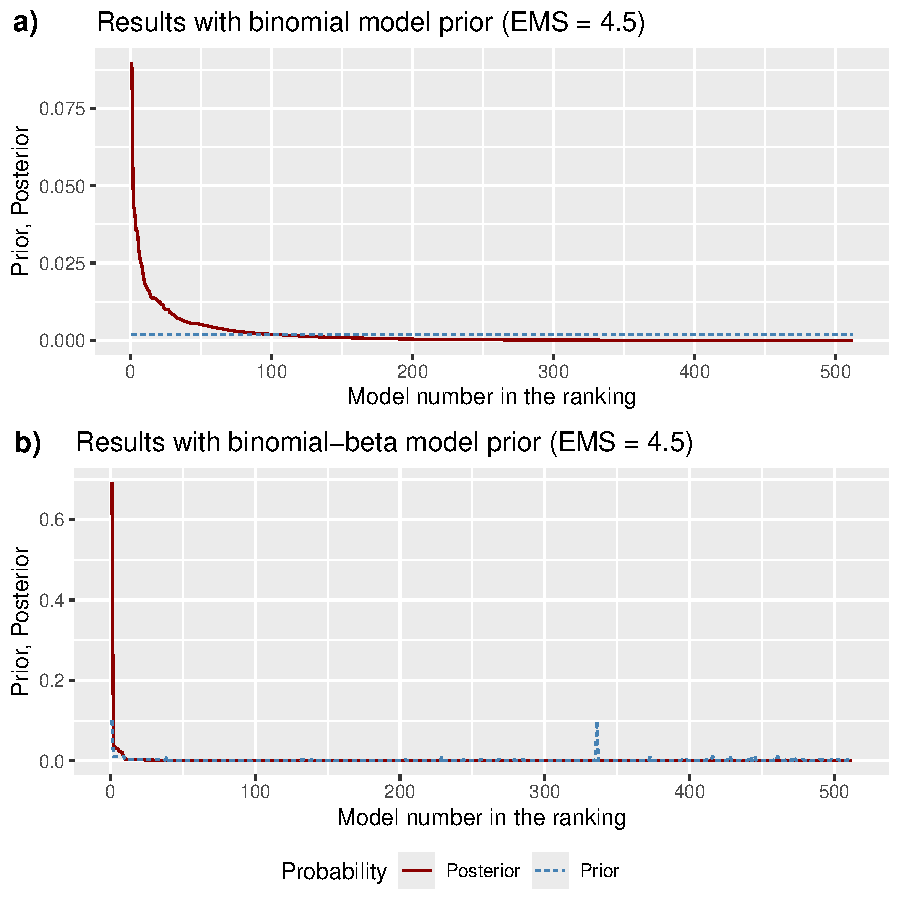
\includegraphics{bdsm_vignette-014}

The graphs demonstrate that most of the posterior probability mass is concentrated within just a couple of models.
To view the results for only the best models, the user can use the \verb+top+ parameter.

\begin{Schunk}
\begin{Sinput}
> for_models <- model_pmp(bma_results, top = 10)
\end{Sinput}
\end{Schunk}
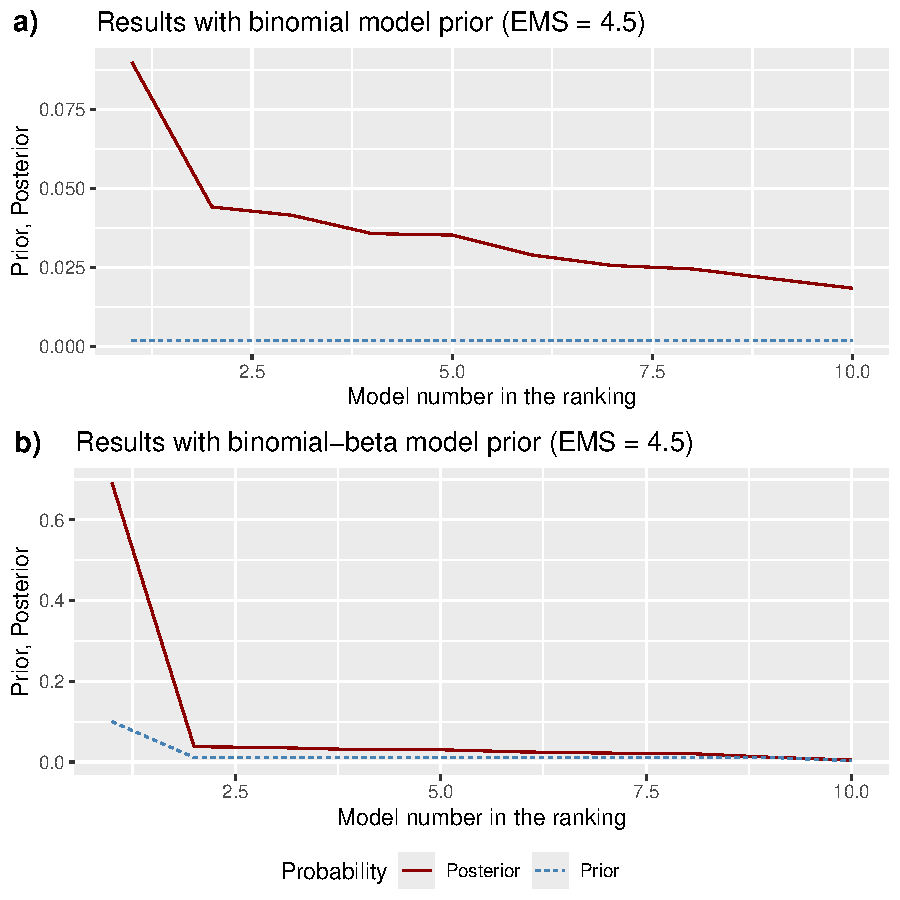
\includegraphics{bdsm_vignette-015}

The last graph for the binomial-beta prior is particularly illuminating in terms of explaining the very high values of posterior inclusion probabilities.
Almost 70\% of the posterior probability mass is concentrated in just one model; therefore, variables included in this model will have very high PIP values.
The model in question will be identified after implementing \verb+model_sizes+ (and \verb+best_models+, which is covered in \autoref{best-models}).
Nevertheless, the results from the graph suggest that the best model is the one that includes all the regressors or none
(because the prior value is around $\frac{1}{9}$ on the plot).

The \verb+model_sizes+ function displays prior and posterior model probabilities on a graph for models of different sizes.
The graphs exclude the lagged dependent variable; therefore, the model with zero regressors still includes the lagged dependent variable.
Similarly to the \verb+model_pmp+ function is returns a list with three objects:
\begin{enumerate}
    \item a graph for the binomial model prior;
    \item a graph for the binomial-beta model prior;
    \item a combined graph for both binomial and binomial-beta model priors.
\end{enumerate}
Again, the user can retrieve each graph separately from the list; however, the function automatically displays a combined graph.

\begin{Schunk}
\begin{Sinput}
> size_graphs <- model_sizes(bma_results)
\end{Sinput}
\end{Schunk}
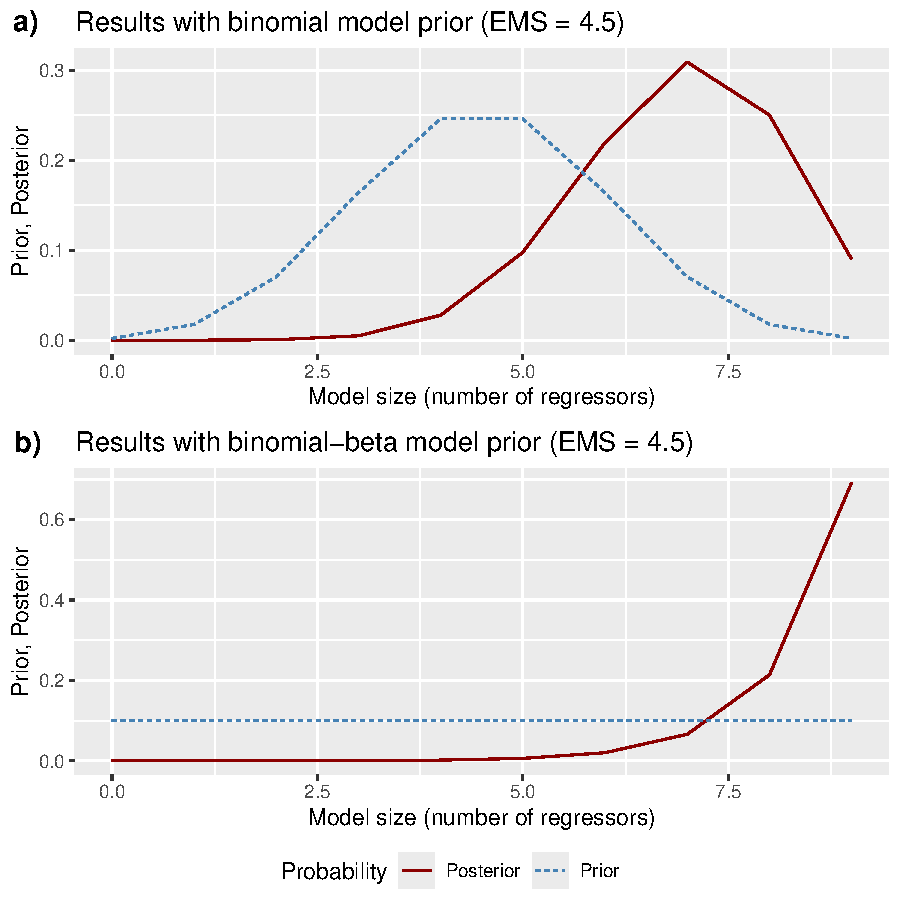
\includegraphics{bdsm_vignette-016}

The graph in panel b) again explains why PIPs are so high in the case of the binomial-beta model prior.
The model with all the regressors accounts for almost 70\% of the total posterior probability mass,
while the remaining portion is concentrated on models with a high number of regressors.
In contrast, the posterior probability mass for the binomial model prior is centered around models with seven regressors.
This graph clearly illustrates the impact of changes in the model prior on posterior probabilities.

\subsection{Selecting the best models}\label{best-models}

The \verb+best_models+ function allows the user to view a chosen number of the best models in terms of posterior model probability.
The function returns a list containing nine objects:
\begin{enumerate}
    \item An inclusion table stored as an array object;
    \item A table with estimation results using regular standard errors, stored as an array object;
    \item A table with estimation results using robust standard errors, stored as an array object;
    \item An inclusion table stored as a knitr object;
    \item A table with estimation results using regular standard errors, stored as a knitr object;
    \item A table with estimation results using robust standard errors, stored as a knitr object;
    \item An inclusion table stored as a gTree object;
    \item A table with estimation results using regular standard errors, stored as a gTree object;
    \item A table with estimation results using robust standard errors, stored as a gTree object;
\end{enumerate}
The parameters \verb+estimate+ and \verb+robust+ pertain only to the results that will be automatically displayed after running the function.
The parameter \verb+criterion+ determines whether the models should be ranked according to posterior model probabilities calculated using the binomial (1) or binomial-beta (2) model prior.
To obtain the inclusion array for the 10 best models ranked with the binomial model prior, the user needs to run:

\begin{Schunk}
\begin{Sinput}
> best_8_models <- best_models(bma_results, criterion = 1, best = 8)
> best_8_models[[1]]
\end{Sinput}
\begin{Soutput}
        'No. 1' 'No. 2' 'No. 3' 'No. 4' 'No. 5' 'No. 6' 'No. 7' 'No. 8'
gdp_lag    1.00   1.000   1.000   1.000   1.000   1.000   1.000   1.000
ish        1.00   1.000   1.000   1.000   1.000   1.000   1.000   0.000
sed        1.00   1.000   1.000   0.000   1.000   1.000   1.000   1.000
pgrw       1.00   1.000   1.000   1.000   0.000   1.000   1.000   1.000
pop        1.00   1.000   1.000   1.000   1.000   1.000   1.000   1.000
ipr        1.00   0.000   1.000   1.000   1.000   1.000   1.000   1.000
opem       1.00   1.000   1.000   1.000   1.000   1.000   0.000   1.000
gsh        1.00   1.000   1.000   1.000   1.000   0.000   1.000   1.000
lnlex      1.00   1.000   1.000   1.000   1.000   1.000   1.000   1.000
polity     1.00   1.000   0.000   1.000   1.000   1.000   1.000   1.000
PMP        0.09   0.044   0.042   0.036   0.035   0.029   0.026   0.025
\end{Soutput}
\end{Schunk}

1 indicates the presence of a given regressor in a model, while the last row displays the posterior model probability of that model.
To obtain a knitr table with estimation output with regular standard errors for best 3 models ranked with binomial-beta model prior, the user needs to run:

\begin{Schunk}
\begin{Sinput}
> best_3_models <- best_models(bma_results, criterion = 2, best = 3)
> best_3_models[[5]]
\end{Sinput}
\begin{Soutput}
|        |      'No. 1'      |      'No. 2'      |      'No. 3'      |
|:-------|:-----------------:|:-----------------:|:-----------------:|
|gdp_lag | 0.924 (0.075)***  | 0.892 (0.073)***  |  0.92 (0.055)***  |
|ish     |  0.077 (0.03)**   | 0.092 (0.029)***  |  0.055 (0.029)*   |
|sed     |   0.053 (0.055)   |   0.007 (0.059)   |  0.081 (0.049)*   |
|pgrw    |   0.025 (0.032)   |   0.017 (0.032)   |   0.037 (0.032)   |
|pop     |  0.095 (0.055)*   | 0.139 (0.053)***  |  0.106 (0.053)**  |
|ipr     |  -0.047 (0.025)*  |        NA         | -0.061 (0.023)*** |
|opem    |   0.036 (0.023)   |   0.032 (0.023)   |  0.041 (0.023)*   |
|gsh     |  -0.019 (0.041)   |   -0.024 (0.04)   |  -0.022 (0.045)   |
|lnlex   |  0.124 (0.058)**  |   0.054 (0.058)   |  0.132 (0.054)**  |
|polity  | -0.083 (0.029)*** | -0.093 (0.029)*** |        NA         |
|PMP     |       0.692       |       0.038       |       0.035       |
\end{Soutput}
\end{Schunk}

The comparison of the last two tables further highlights the importance of the model prior.
The best model under the binomial model prior accounts for around 9\% of the posterior probability mass,
while the best model under the binomial-beta model prior accounts for over 69\%.
Finally, to obtain a gTree table with estimation output using robust standard errors for the top 3 models ranked by the binomial-beta model prior,
the user needs to run:

\begin{Schunk}
\begin{Sinput}
> best_3_models <- best_models(bma_results, criterion = 2, best = 3)
> best_3_models[[9]]
\end{Sinput}
\begin{Soutput}
gTree[GRID.gTree.2013] 
\end{Soutput}
\end{Schunk}
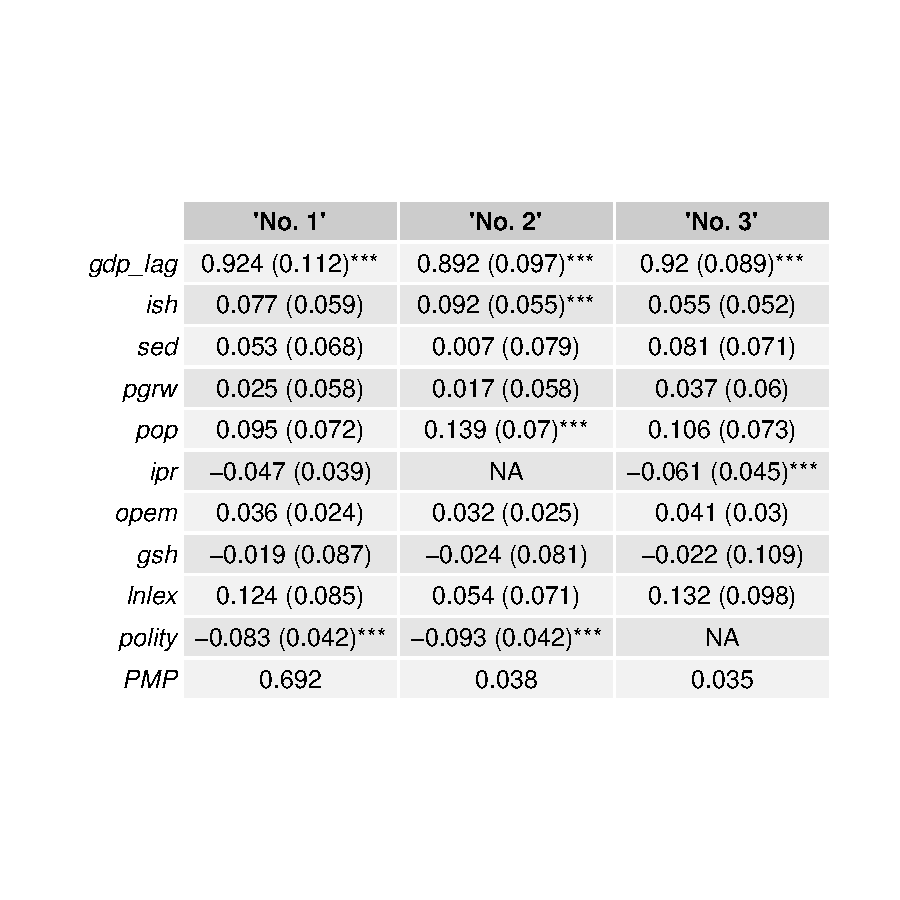
\includegraphics{bdsm_vignette-019}

The comparison of the last two tables and the estimation outputs with regular and robust standard errors demonstrates
how the results change when switching between these two variance estimators.

\subsection{Calculating jointness measures}

Within the BMA framework, it is possible to establish the nature of the relationship between pairs of examined regressors using the jointness measures.
This can be accomplished using the \verb+jointness+ function.
The latest jointness measure, introduced by \citet{Hofmarcher+2018}, has been shown to outperform older alternatives developed by \citet{Ley+2007} and \citet{Doppelhofer+2009}\footnote{See section \ref{prior_joint} for the interpretations of jointness measures.}.
Therefore, the \citet{Hofmarcher+2018} measure is the default option in the \verb+jointness+ function.

\begin{Schunk}
\begin{Sinput}
> jointness(bma_results)
\end{Sinput}
\begin{Soutput}
         ish   sed  pgrw   pop   ipr  opem   gsh lnlex polity
ish       NA 0.217 0.208 0.531 0.151 0.262 0.244 0.366  0.182
sed    0.806    NA 0.155 0.421 0.116 0.200 0.189 0.289  0.126
pgrw   0.806 0.779    NA 0.416 0.124 0.199 0.187 0.284  0.132
pop    0.906 0.874 0.874    NA 0.304 0.517 0.490 0.711  0.346
ipr    0.782 0.758 0.759 0.846    NA 0.153 0.139 0.210  0.102
opem   0.830 0.802 0.803 0.902 0.781    NA 0.241 0.373  0.170
gsh    0.822 0.795 0.795 0.894 0.773 0.820    NA 0.341  0.154
lnlex  0.865 0.836 0.836 0.944 0.811 0.863 0.854    NA  0.227
polity 0.791 0.764 0.765 0.856 0.745 0.788 0.780 0.818     NA
\end{Soutput}
\end{Schunk}

\noindent Above the main diagonal the user can find the results for the binomial model prior, and below the results for the binomial-beta model prior.
All the values in the table are positive, indicating complementary relationships between the regressors.
Notably, the values for the binomial-beta prior are substantially higher than those for the binomial prior.
This result is not surprising, as the model with all the regressors accounts for almost $70\%$ of the total posterior probability mass.

To obtain the results for the \citet{Ley+2007} measure, the user should run:

\begin{Schunk}
\begin{Sinput}
> jointness(bma_results, measure = "LS")
\end{Sinput}
\begin{Soutput}
          ish    sed   pgrw    pop   ipr   opem    gsh  lnlex polity
ish        NA  1.470  1.448  3.285 1.230  1.678  1.603  2.213  1.324
sed     9.551     NA  1.250  2.467 1.091  1.424  1.378  1.812  1.141
pgrw    9.539  8.284     NA  2.437 1.100  1.416  1.369  1.792  1.146
pop    20.258 14.941 14.953     NA 1.876  3.162  2.935  5.986  2.062
ipr     8.387  7.441  7.492 12.022    NA  1.223  1.178  1.477  1.014
opem   11.040  9.361  9.375 19.533 8.307     NA  1.583  2.212  1.292
gsh    10.492  8.999  9.012 17.822 7.998 10.341     NA  2.061  1.241
lnlex  14.094 11.424 11.425 35.099 9.745 13.898 12.960     NA  1.566
polity  8.777  7.686  7.724 12.875 7.014  8.630  8.293 10.198     NA
\end{Soutput}
\end{Schunk}

\noindent The values corroborate the results obtained using the \citet{Hofmarcher+2018} measure.
All the regressors exhibit complementary relationships, which are visibly stronger under the binomial-beta model prior.

However, the \citet{Doppelhofer+2009} measure yields a slightly different outcome:

\begin{Schunk}
\begin{Sinput}
> jointness(bma_results, measure = "DW")
\end{Sinput}
\begin{Soutput}
         ish   sed   pgrw    pop    ipr   opem   gsh  lnlex polity
ish       NA 0.051  0.020  0.005  0.018  0.030 0.008 -0.004  0.067
sed    0.989    NA -0.023 -0.029  0.004 -0.008 0.000  0.005 -0.024
pgrw   0.974 0.905     NA -0.001  0.047 -0.001 0.001 -0.007  0.010
pop    1.019 0.957  0.987     NA -0.018 -0.023 0.049  0.154  0.012
ipr    0.985 0.931  0.980  0.974     NA  0.048 0.019  0.025  0.036
opem   1.012 0.938  0.949  0.991  1.006     NA 0.032  0.139  0.032
gsh    0.972 0.931  0.941  1.042  0.962  0.991    NA  0.034  0.001
lnlex  0.983 0.957  0.954  1.173  0.985  1.105 1.001     NA -0.056
polity 1.013 0.903  0.939  0.994  0.967  0.980 0.934  0.906     NA
\end{Soutput}
\end{Schunk}

\noindent In this case, some pairs of regressors have negative values of the jointness measure under the binomial model prior;
however, these values are very close to zero, indicating unrelated variables.
Once again, the values for the binomial-beta model prior are higher, demonstrating how the results are influenced by the choice of model prior.

\subsection{Visualizing model coefficients}

The \verb+coef_hist+ function allows the user to plot the distribution of estimated coefficients.
It returns a list containing a number of objects equal to the number of regressors plus one.
The first object in the list is a graph of the coefficients for the lagged dependent variable, while the remaining objects are graphs of the coefficients for the other regressors.
The graph for the lagged dependent variable collects coefficients from the entire model space, whereas the graphs for the other regressors only collect coefficients from the models that include the given regressor (half of the model space).

There are two main options for visualizing the coefficient distributions.
The first option uses a histogram.
The \verb+coef_hist+ function provides the user with options for controlling the bin widths of the histogram (\verb+BW+, \verb+binW+, \verb+BN+, and \verb+num+).
The default is \verb+BW = FD+, which selects bin widths using the Freedman-Diaconis method.
\begin{Schunk}
\begin{Sinput}
> coef_plots <- coef_hist(bma_results)
> coef_plots[[1]]
\end{Sinput}
\end{Schunk}
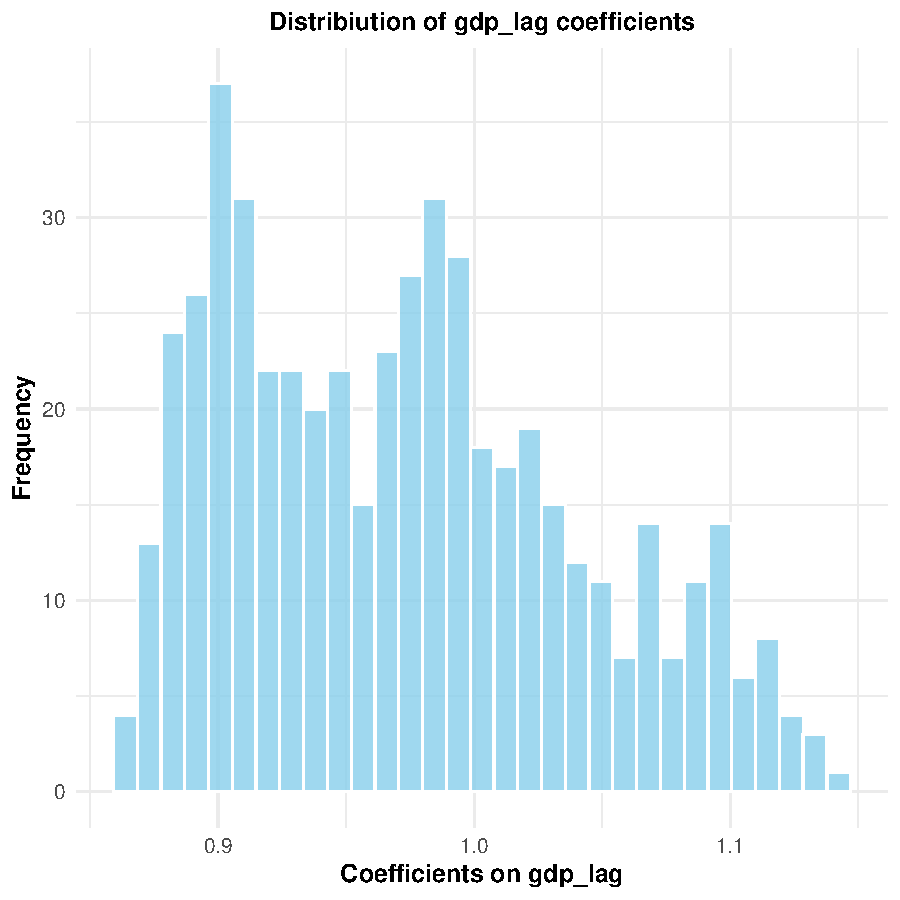
\includegraphics{bdsm_vignette-023}

The second option allows the user to plot kernel densities.
\begin{Schunk}
\begin{Sinput}
> coef_plots2 <- coef_hist(bma_results, kernel = 1)
> coef_plots2[[1]]
\end{Sinput}
\end{Schunk}
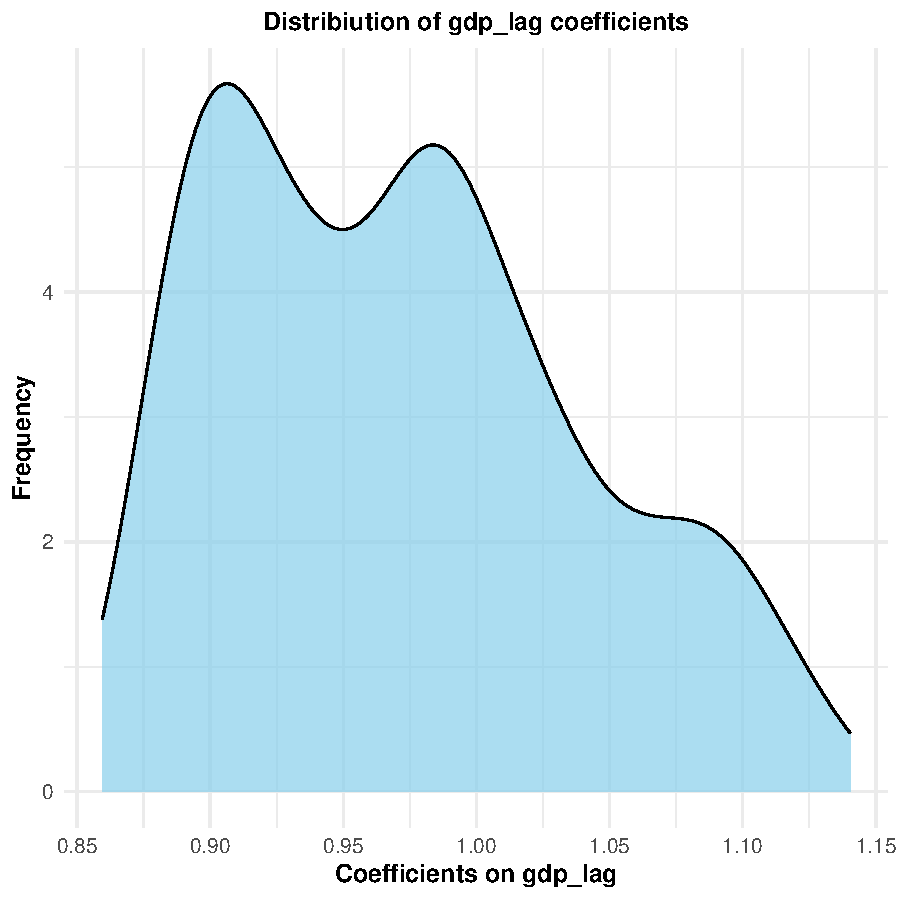
\includegraphics{bdsm_vignette-024}

The choice of appropriate plotting options is left to the user's preferences regarding the style of presentation and the size of the model space.
\begin{Schunk}
\begin{Sinput}
> library(gridExtra)
> grid.arrange(coef_plots[[1]], coef_plots[[2]], coef_plots2[[1]],
+              coef_plots2[[2]], nrow = 2, ncol = 2)
\end{Sinput}
\end{Schunk}
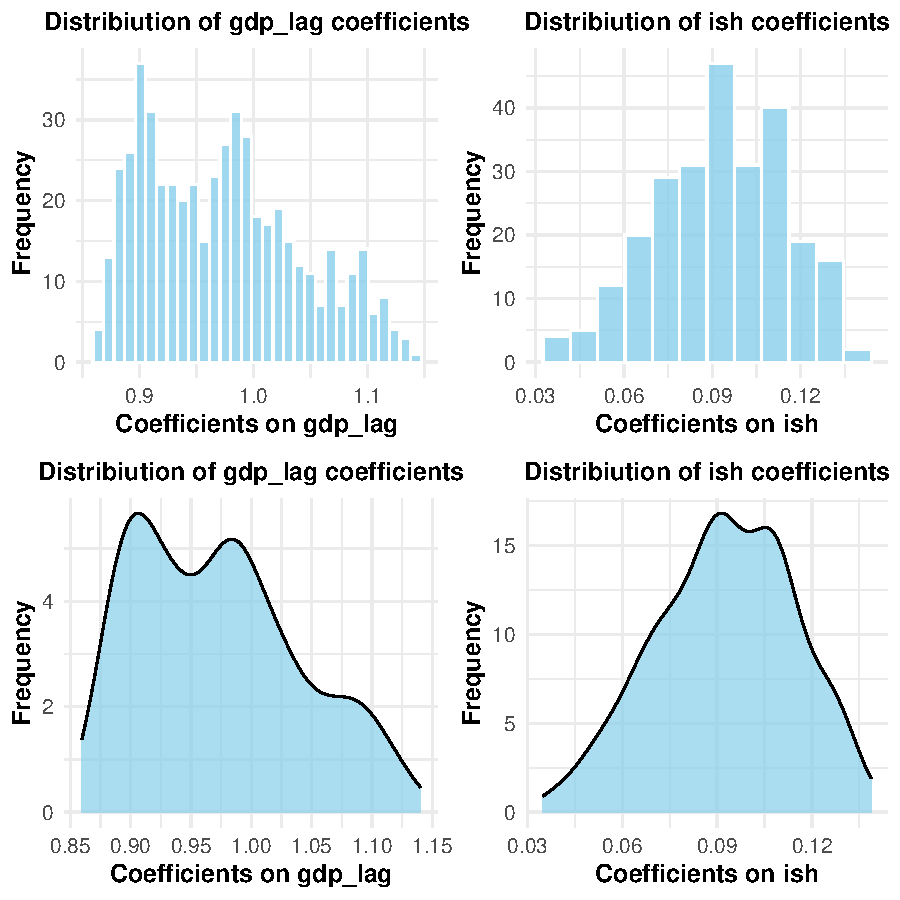
\includegraphics{bdsm_vignette-025}

\section{Changes in model priors}\label{priors}

This section provides a more detailed description of the available model prior options.
Subsection \ref{ems} discusses the consequences of changes in the expected model size, while subsection \ref{dil} describes the dilution prior.

\subsection{Changing expected model size}\label{ems}

The \verb+bma+ function calculates BMA statistics using both the binomial and binomial-beta model priors.
By default, the \verb+bma+ function sets the expected model size (EMS) to $K/2$, where $K$ denotes the total number of regressors.
The binomial model prior with $EMS = K/2$ leads to a uniform model prior, assigning equal probabilities to all models.
In contrast, the binomial-beta model prior with $EMS = K/2$ assumes equal probabilities across all model sizes.
However, the user can modify the prior model specification by changing the \verb+EMS+ parameter.

First, consider the consequence of concentrating prior probability mass on small models by setting $EMS = 2$.

\begin{Schunk}
\begin{Sinput}
> bma_results2 <- bma(bma_prep_objects_full, df = data_prepared,
+                     round = 3, EMS = 2)
\end{Sinput}
\end{Schunk}

\noindent Before turning to the main BMA results, let us focus on the changes in the posterior probability mass with respect to model sizes.

\begin{Schunk}
\begin{Sinput}
> bma_results2[[16]]
\end{Sinput}
\begin{Soutput}
              Prior models size Posterior model size
Binomial                      2                4.560
Binomial-beta                 2                7.502
\end{Soutput}
\end{Schunk}

\noindent The results show that decreasing the prior expected model size led to a considerable decline in the posterior expected model size.
The consequences of this change in the prior expected model size are best illustrated using the prior and posterior probability mass over model sizes.

\begin{Schunk}
\begin{Sinput}
> size_graphs2 <- model_sizes(bma_results2)
\end{Sinput}
\end{Schunk}
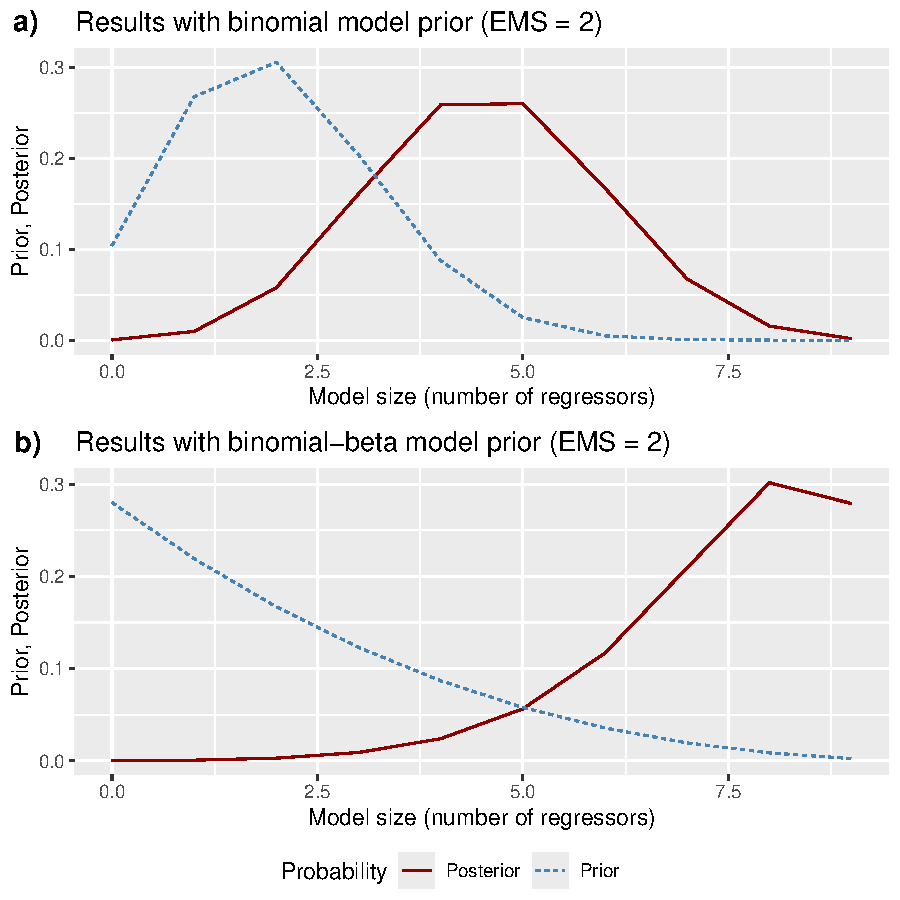
\includegraphics{bdsm_vignette-028}

For both the binomial and binomial-beta model priors, the prior probability mass is more concentrated on small model sizes.
However, for the binomial model prior, the center of the posterior probability mass shifted to medium-sized models, while it remained on large models for the binomial-beta model prior.
Nevertheless, the posterior model probability for the model with all regressors decreased from nearly 0.7 for $EMS = 4.5$ to less than 0.3.
There are also substantial changes in the distribution of the posterior probability mass over the model space.
\begin{Schunk}
\begin{Sinput}
> model_graphs2 <- model_pmp(bma_results2)
\end{Sinput}
\end{Schunk}
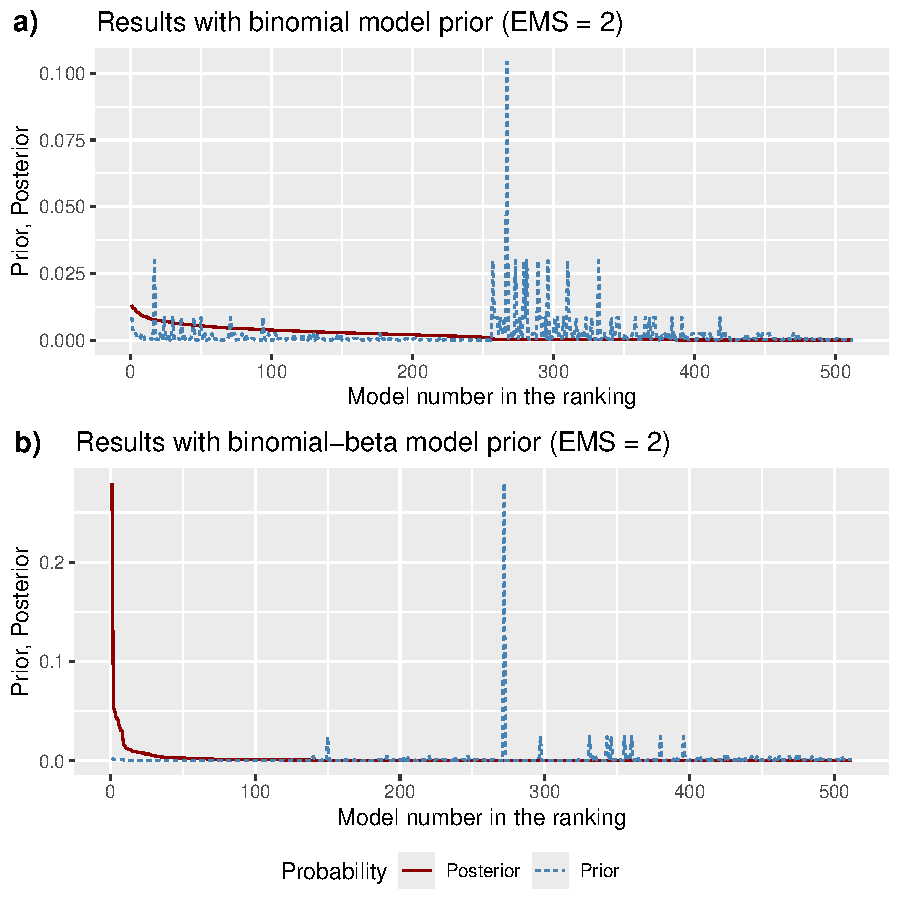
\includegraphics{bdsm_vignette-029}

Both panels of the graph show that the prior and posterior model probabilities have substantially decoupled from each other.
This strongly indicates that the prior and the data are suggesting vastly different model choices.
The tall blue spike represents the model with no regressors.
The main BMA posterior statistic for the binomial model prior also experienced a significant change.
\begin{Schunk}
\begin{Sinput}
> bma_results2[[1]]
\end{Sinput}
\begin{Soutput}
          PIP     PM   PSD  PSDR  PMcon PSDcon PSDRcon    %(+)
gdp_lag    NA  0.925 0.080 0.102  0.925  0.080   0.102 100.000
ish     0.483  0.043 0.050 0.059  0.088  0.034   0.057 100.000
sed     0.420  0.014 0.046 0.058  0.034  0.065   0.085  70.312
pgrw    0.414  0.009 0.025 0.041  0.022  0.034   0.061  99.609
pop     0.964  0.142 0.065 0.082  0.147  0.060   0.078 100.000
ipr     0.344 -0.019 0.031 0.037 -0.056  0.028   0.045   0.000
opem    0.468  0.024 0.032 0.033  0.052  0.026   0.030 100.000
gsh     0.459 -0.003 0.032 0.071 -0.007  0.047   0.105  28.906
lnlex   0.637  0.052 0.068 0.087  0.082  0.069   0.096 100.000
polity  0.372 -0.029 0.042 0.046 -0.079  0.031   0.043   0.000
\end{Soutput}
\end{Schunk}

\noindent Posterior inclusion probabilities drop considerably for all the regressors, except for population, which remains almost unchanged.
Interestingly, the ratios for all variables declined, with population being the exception.
The ratio for population remains above two for regular standard errors and 1.7 for robust standard errors.
This outcome indicates that population performs relatively better in smaller models.
The results for binomial-beta model prior are  given below.
\begin{Schunk}
\begin{Sinput}
> bma_results2[[2]]
\end{Sinput}
\begin{Soutput}
          PIP     PM   PSD  PSDR  PMcon PSDcon PSDRcon    %(+)
gdp_lag    NA  0.919 0.075 0.109  0.919  0.075   0.109 100.000
ish     0.838  0.067 0.042 0.061  0.080  0.033   0.059 100.000
sed     0.796  0.037 0.057 0.071  0.047  0.061   0.077  70.312
pgrw    0.795  0.020 0.031 0.054  0.025  0.033   0.059  99.609
pop     0.992  0.114 0.061 0.078  0.115  0.061   0.078 100.000
ipr     0.754 -0.037 0.031 0.042 -0.049  0.026   0.042   0.000
opem    0.833  0.034 0.028 0.030  0.041  0.025   0.028 100.000
gsh     0.822 -0.015 0.040 0.087 -0.018  0.043   0.095  28.906
lnlex   0.902  0.097 0.071 0.094  0.107  0.066   0.093 100.000
polity  0.769 -0.064 0.044 0.051 -0.083  0.030   0.043   0.000
\end{Soutput}
\end{Schunk}

\noindent The change in PIPs is again significant, though not as pronounced as in the case of the binomial model prior.
Changes in the ratios are relatively small and irregular for both regular and robust standard errors.
The most pronounced change is the drop in the value of the ratios for the democracy index (\verb+polity+), indicating that this regressor performs better in larger models.

It is also very instructive to examine the jointness measures calculated under the new prior specification.
\begin{Schunk}
\begin{Sinput}
> jointness(bma_results2, measure = "HCGHM", rho = 0.5, round = 3)
\end{Sinput}
\begin{Soutput}
         ish   sed  pgrw    pop    ipr   opem    gsh  lnlex polity
ish       NA 0.021 0.008 -0.030  0.003  0.002  0.001 -0.012  0.021
sed    0.441    NA 0.017 -0.146  0.043  0.007  0.011 -0.036  0.026
pgrw   0.437 0.390    NA -0.155  0.053  0.012  0.011 -0.041  0.037
pop    0.667 0.586 0.583     NA -0.281 -0.057 -0.072  0.253 -0.231
ipr    0.391 0.355 0.361  0.503     NA  0.021  0.023 -0.065  0.072
opem   0.483 0.430 0.430  0.657  0.391     NA  0.010  0.022  0.020
gsh    0.467 0.419 0.418  0.636  0.378  0.464     NA -0.012  0.019
lnlex  0.559 0.497 0.495  0.793  0.439  0.562  0.538     NA -0.072
polity 0.413 0.364 0.369  0.532  0.340  0.405  0.390  0.453     NA
\end{Soutput}
\end{Schunk}
On the one hand, the results obtained with the binomial-beta model prior did not change in any significant manner.
On the other hand, the results obtained with the binomial model prior changed substantially.
The measure indicates that population is a substitute for both the investment price (\verb+ipr+) and the democracy index, as well as, to a lesser extent, secondary education (\verb+sed+) and population growth (\verb+pgrw+).

Next, to consider the consequences of concentrating prior probability mass on large models, \verb+EMS+ was set to eight.
\begin{Schunk}
\begin{Sinput}
> bma_results8 <- bma(bma_prep_objects_full, df = data_prepared,
+                     round = 3, EMS = 8)
> bma_results8[[16]]
\end{Sinput}
\begin{Soutput}
              Prior models size Posterior model size
Binomial                      8                8.666
Binomial-beta                 8                8.944
\end{Soutput}
\end{Schunk}

\noindent The posterior model size increased for the binomial prior; however, it remained almost unchanged for the binomial-beta model prior.
The most interesting aspect is the new graphs of prior and posterior probability mass over the model sizes.
\begin{Schunk}
\begin{Sinput}
> size_graphs8 <- model_sizes(bma_results8)
\end{Sinput}
\end{Schunk}
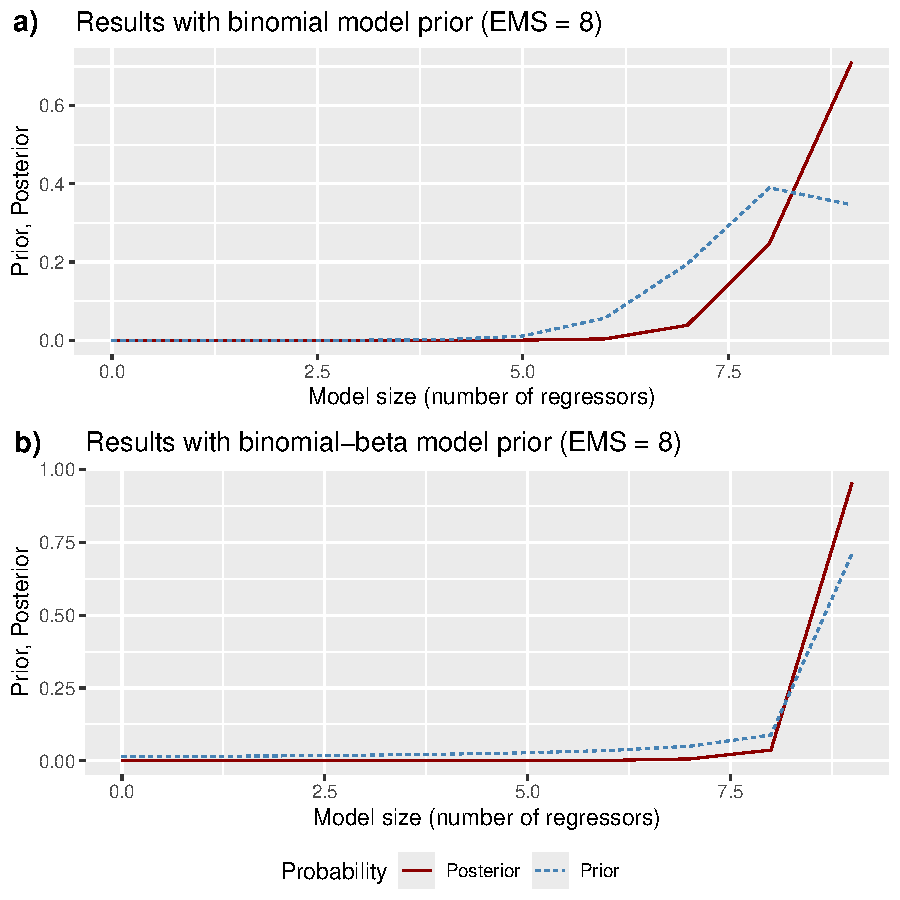
\includegraphics{bdsm_vignette-034}

In both cases, the posterior probability mass has concentrated near the models with all the regressors.
However, in the case of the binomial-beta model prior, the model with all the regressors captures most of the posterior probability mass (almost $96\%$).
This conclusion is further supported by the graphs of posterior model probability across the entire model space.
\begin{Schunk}
\begin{Sinput}
> model_graphs8 <- model_pmp(bma_results8)
\end{Sinput}
\end{Schunk}
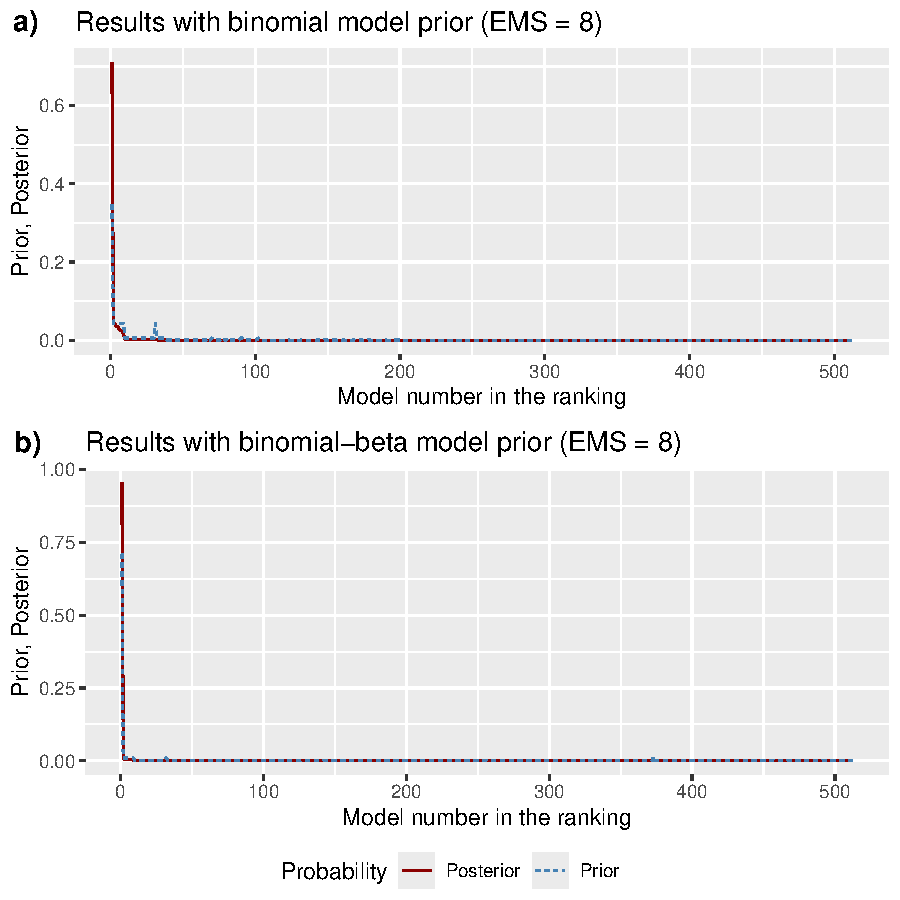
\includegraphics{bdsm_vignette-035}

Panel (a) demonstrates that the change in the expected model size led to a substantial increase in the posterior model probability for the model with all regressors under the binomial model prior.
It now accounts for over $70\%$ of the total posterior probability mass.
The increase in the expected model size also influenced the main BMA statistics.
\begin{Schunk}
\begin{Sinput}
> bma_results8[[1]]
\end{Sinput}
\begin{Soutput}
          PIP     PM   PSD  PSDR  PMcon PSDcon PSDRcon    %(+)
gdp_lag    NA  0.922 0.075 0.112  0.922  0.075   0.112 100.000
ish     0.967  0.075 0.034 0.060  0.077  0.031   0.059 100.000
sed     0.953  0.049 0.057 0.070  0.051  0.057   0.071  70.312
pgrw    0.953  0.024 0.032 0.057  0.025  0.032   0.058  99.609
pop     0.999  0.100 0.057 0.074  0.100  0.057   0.074 100.000
ipr     0.942 -0.045 0.027 0.040 -0.048  0.025   0.040   0.000
opem    0.965  0.036 0.024 0.026  0.037  0.024   0.025 100.000
gsh     0.961 -0.019 0.041 0.088 -0.019  0.042   0.090  28.906
lnlex   0.981  0.117 0.062 0.088  0.119  0.061   0.088 100.000
polity  0.945 -0.078 0.034 0.045 -0.083  0.030   0.043   0.000
\end{Soutput}
\end{Schunk}

\noindent The PIPs increased considerably.
Population is classified as very strong, while the other regressors are classified as strong or positive.
Interestingly, all the ratios have improved as well, except for population.
The change in the results for the binomial-beta model prior is less pronounced.
\begin{Schunk}
\begin{Sinput}
> bma_results8[[2]]
\end{Sinput}
\begin{Soutput}
          PIP     PM   PSD  PSDR  PMcon PSDcon PSDRcon    %(+)
gdp_lag    NA  0.923 0.075 0.112  0.923  0.075   0.112 100.000
ish     0.994  0.076 0.031 0.060  0.077  0.030   0.059 100.000
sed     0.992  0.052 0.055 0.068  0.053  0.055   0.068  70.312
pgrw    0.992  0.025 0.032 0.058  0.025  0.032   0.058  99.609
pop     1.000  0.096 0.055 0.072  0.096  0.055   0.072 100.000
ipr     0.990 -0.047 0.025 0.039 -0.047  0.025   0.039   0.000
opem    0.994  0.036 0.023 0.024  0.036  0.023   0.024 100.000
gsh     0.994 -0.019 0.041 0.087 -0.019  0.041   0.088  28.906
lnlex   0.997  0.123 0.058 0.086  0.123  0.058   0.086 100.000
polity  0.991 -0.082 0.030 0.043 -0.083  0.029   0.042   0.000
\end{Soutput}
\end{Schunk}

\noindent With the increase in expected model size, population is classified as very strong,
and all the other regressors are classified as strong in terms of the posterior inclusion probability criterion.
Similarly to the case of the binomial prior, all the ratios increased except for population.

Again, it is instructive to examine the jointness measures.
\begin{Schunk}
\begin{Sinput}
> jointness(bma_results8, measure = "HCGHM", rho = 0.5, round = 3)
\end{Sinput}
\begin{Soutput}
         ish   sed  pgrw   pop   ipr  opem   gsh lnlex polity
ish       NA 0.840 0.841 0.931 0.819 0.865 0.857 0.896  0.826
sed    0.975    NA 0.814 0.903 0.792 0.837 0.830 0.869  0.799
pgrw   0.975 0.971    NA 0.904 0.793 0.838 0.830 0.870  0.800
pop    0.988 0.984 0.984    NA 0.881 0.928 0.920 0.960  0.888
ipr    0.972 0.968 0.968 0.980    NA 0.816 0.808 0.847  0.778
opem   0.978 0.974 0.974 0.988 0.971    NA 0.854 0.894  0.823
gsh    0.977 0.973 0.973 0.987 0.970 0.977    NA 0.886  0.815
lnlex  0.983 0.979 0.979 0.993 0.976 0.983 0.982    NA  0.854
polity 0.973 0.969 0.969 0.982 0.966 0.972 0.971 0.977     NA
\end{Soutput}
\end{Schunk}

\noindent The values of the measures show that all the regressors exhibit a very strong complementary relationship.
This outcome, once again, underscores the importance of carefully considering the prior when interpreting jointness measures.

\subsection{Dilution prior}\label{dil}
One of the main issues associated with identifying robust regressors is multicollinearity.
Some regressors may approximate the same underlying factor influencing the dependent variable.
Multicollinearity may result from the absence of observable variables associated with a specific theory or from a theory failing to provide a unique candidate for a regressor.
Moreover, some regressors may share a common determinant.
Although \citet{Moral+2013, Moral+2016} addressed this issue to some extent, researchers have another option to mitigate multicollinearity: the dilution prior proposed by \citet{George+2010} which was described in detail in \autoref{prior_joint}.

To apply the dilution prior, the user must set \verb+dilution = 1+ in the \verb+bma+ function.
The user can also manipulate the dilution parameter $\omega$.
The default option is \verb+dil.Par = 0.5+, as recommended by \citet{George+2010}.
\begin{Schunk}
\begin{Sinput}
> bma_results_dil <- bma(bma_prep_objects_full, df = data_prepared,
+                        round = 3, dilution = 1)
\end{Sinput}
\end{Schunk}

\noindent The effect of implementing the dilution prior is well depicted by the distribution of prior probability mass over the model sizes.

\begin{Schunk}
\begin{Sinput}
> size_graphs_dil <- model_sizes(bma_results_dil)
\end{Sinput}
\end{Schunk}
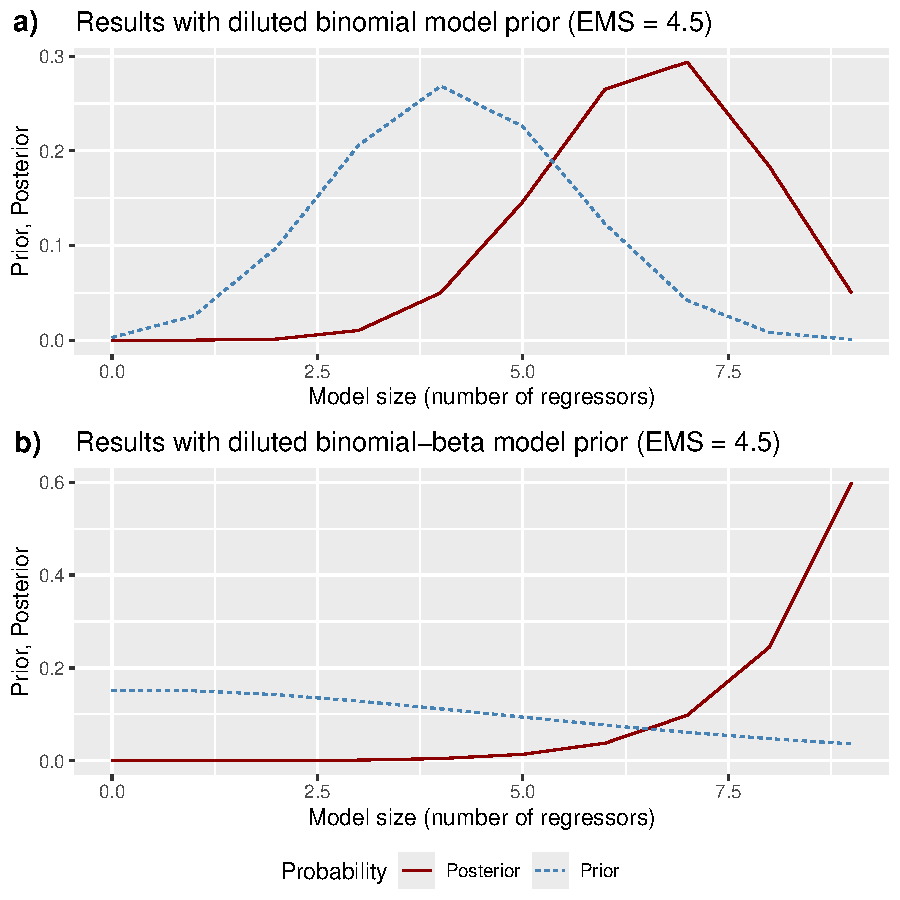
\includegraphics{bdsm_vignette-040}

The change in the prior distribution is more visible for the binomial-beta model prior.
In panel b, the prior probability mass has decreased for larger models and increased for smaller models.
However, this change is not uniform, as models characterized by the highest degree of multicollinearity are subject to the greatest penalty in terms of prior probability mass.

Before moving to the BMA statistics, it is instructive to examine the change in the \verb+dil.Par+ parameter.
\begin{Schunk}
\begin{Sinput}
> bma_results_dil01 <- bma(bma_prep_objects_full, df = data_prepared,
+                        round = 3, dilution = 1, dil.Par = 0.1)
> size_graphs_dil01 <- model_sizes(bma_results_dil01)
\end{Sinput}
\end{Schunk}
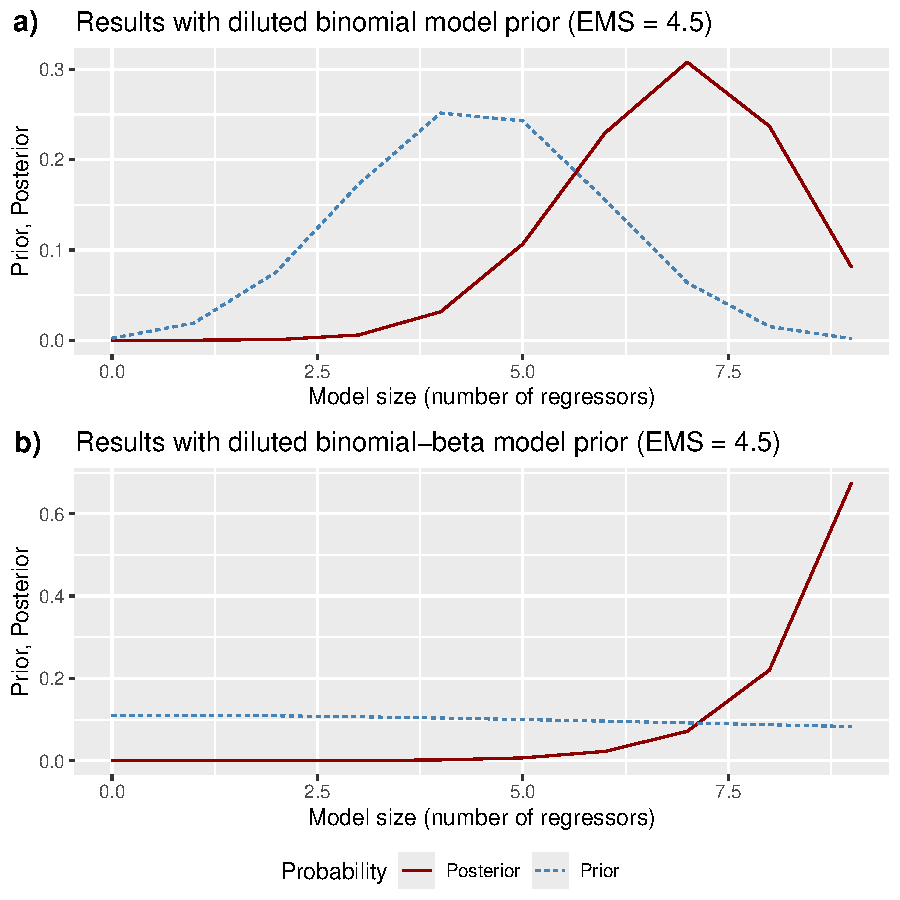
\includegraphics{bdsm_vignette-041}

\noindent As we can see, decreasing the value of $\omega$ diminishes the impact of dilution on the model prior.
Conversely, raising the \verb+dil.Par+ parameter increases the degree of dilution.
\begin{Schunk}
\begin{Sinput}
> bma_results_dil2 <- bma(bma_prep_objects_full, df = data_prepared,
+                        round = 3, dilution = 1, dil.Par = 2)
> size_graphs_dil2 <- model_sizes(bma_results_dil2)
\end{Sinput}
\end{Schunk}
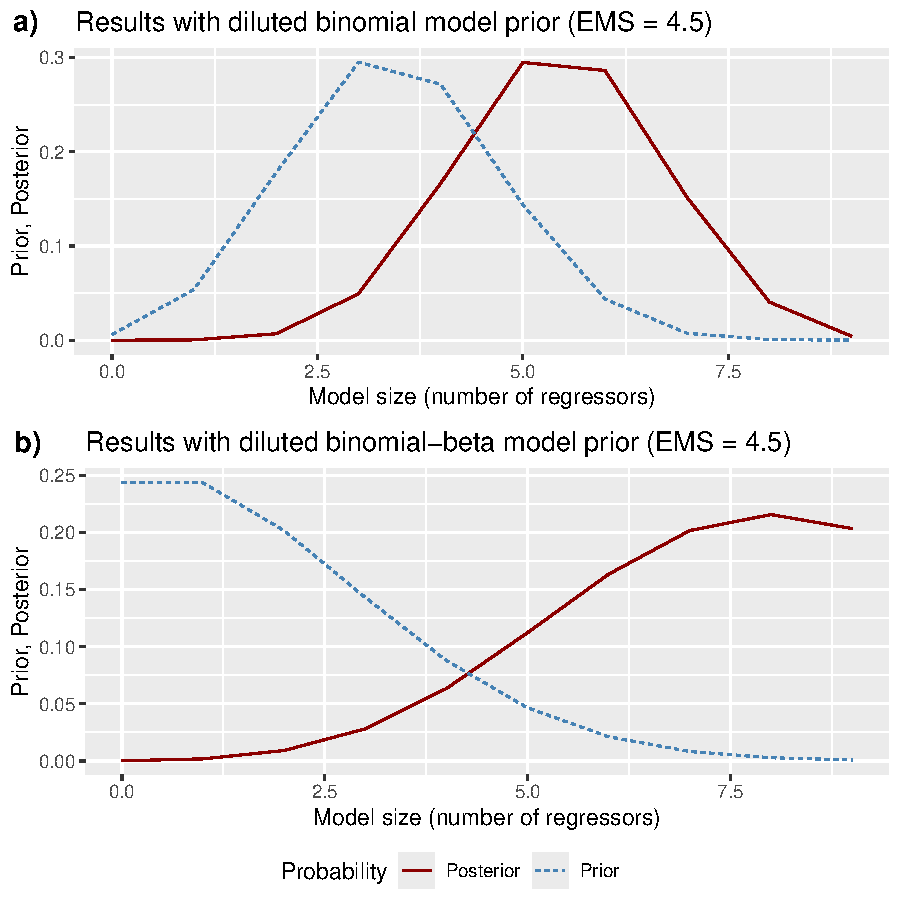
\includegraphics{bdsm_vignette-042}

\noindent An especially strong impact can be seen for the binomial-beta prior.

However, even after giving such priority to the penalty for multicollinearity,
the main BMA statistics remain stable.
\begin{Schunk}
\begin{Sinput}
> bma_results_dil2[[2]]
\end{Sinput}
\begin{Soutput}
          PIP     PM   PSD  PSDR  PMcon PSDcon PSDRcon    %(+)
gdp_lag    NA  0.924 0.076 0.107  0.924  0.076   0.107 100.000
ish     0.735  0.056 0.044 0.060  0.076  0.033   0.058 100.000
sed     0.641  0.029 0.054 0.067  0.046  0.062   0.078  70.312
pgrw    0.687  0.019 0.030 0.052  0.028  0.033   0.060  99.609
pop     0.993  0.121 0.064 0.080  0.122  0.063   0.080 100.000
ipr     0.773 -0.039 0.032 0.044 -0.050  0.027   0.044   0.000
opem    0.824  0.037 0.029 0.031  0.045  0.026   0.029 100.000
gsh     0.840 -0.014 0.042 0.094 -0.017  0.045   0.102  28.906
lnlex   0.767  0.086 0.075 0.097  0.112  0.066   0.097 100.000
polity  0.613 -0.050 0.046 0.052 -0.081  0.030   0.043   0.000
\end{Soutput}
\end{Schunk}
Hence, we see that \citet{Moral+2016}’s claim about the fragility of growth regressors withstands the test of various manipulations in the model prior.

\section{Concluding remarks}\label{sum}

This manuscript introduces the \verb+bdsm+ package, which enables Bayesian model averaging for dynamic panels with weakly exogenous regressors — a methodology developed by \citet{Moral+2012,Moral+2013,Moral+2016}.
This package allows researchers to simultaneously address model uncertainty and reverse causality and is the only \verb+R+ package offering these capabilities.
It provides flexible options for specifying model priors, including dilution prior that accounts for multicollinearity.
The package also includes graphical tools for visualizing prior and posterior model probabilities across model space and model sizes, as well as functions for plotting histograms and kernel densities of the estimated coefficients.
Additionally, it allows researchers to compute jointness measures introduced by \citet{Doppelhofer+2009,Ley+2007,Hofmarcher+2018} to assess whether pairs of regressors act as substitutes or complements.
Users can also perform Bayesian model selection to examine in detail the most probable models based on posterior model probability.

The manuscript outlines the methodological approach, while the detailed explanation can be found in \citet{Moral+2012,Moral+2013,Moral+2016}.
Users unfamiliar with this approach can easily learn to apply it through the hands-on tutorial provided in the manuscript.
The package’s functionalities are illustrated using the original dataset from \citet{Moral+2016} in the context of analyzing the determinants of economic growth.
The results of the examination illustrate that fragility of growth determinants is a persistent feature of the data, confirming \citet{Moral+2016} claims.
The various empirical exercises underscore two important aspects of any BMA analysis.
First, the results should always be validated through extensive changes in prior specifications.
Second, the robustness of the regressors must be evaluated using both
posterior inclusion probabilities and the ratios of the posterior mean to the posterior standard deviation,
as these measures can often lead to differing conclusions.


\addcontentsline{toc}{section}{References}
\bibliography{references}
\bibliographystyle{apalike}

\end{document}
